% Chapter, Section, Figure, Table, Theorem, Corollary, Lemma, Definition, {\bf 
\chapter{Regular Grammars}\label{ch-8}

In the preceding chapters, we have seen several ways to characterize the set
of FAD languages: via DFAs, NDFAs, right congruences, and regular expressions.
In this chapter we will look at still another way to represent this class, using
the concept of \emph{\Index{grammars}}. This construct is very powerful, and
many restrictions must be placed on the general definition of a grammar in order
to limit the scope to FAD languages. The very restrictive \emph{regular}
grammars will be explored in full detail in this chapter. The more robust
classes of grammars introduced here will be discussed at length in later
chapters.

\section{Overview Of The Grammar Hierarchy}\label{sec-8.1}

Much like the rules given in Backus-Naur Form (BNF) in Chapters \ref{ch-0} and \ref{ch-1}, the
language-defining power of a grammar stems from the generation of strings
through the successive replacement of symbols in a partially constructed string.
These replacement rules form the foundation for the definition of programming
languages and are used in compiler construction not only to determine correct
syntax, but also to help determine the \emph{meaning} of the statements and
thereby guide the translation of a program into machine language.

\subsection*{Example 8.1}

A BNF that describes the set of all valid FORTRAN identifiers is given below.
Recall that such identifiers must begin with a letter and be followed by no
more than five other letters and numerals. These criteria can be specified by
the following set of rules.
\begin{center}\begin{tabular}{r@{:: = }l}
$S$ & $\pmb{a}S_1|\pmb{b}S_1| \ldots |\pmb{z}S_1|\pmb{a}|\pmb{b}| \ldots
	|\pmb{z}$ \\
$S_1$ & $\pmb{a}S_2|\pmb{b}S_2| \ldots |\pmb{z}S_2|\pmb{a}|\pmb{b}| \ldots
	|\pmb{z}|\pmb{0}S_2|\pmb{1}S_2|\pmb{2}S_2| \ldots |\pmb{9}S_2|\pmb{0}|
	\pmb{1}|\pmb{2}| \ldots |\pmb{9}$ \\
$S_2$ & $\pmb{a}S_3|\pmb{b}S_3| \ldots |\pmb{z}S_3|\pmb{a}|\pmb{b}| \ldots
	|\pmb{z}|\pmb{0}S_3|\pmb{1}S_3|\pmb{2}S_3| \ldots |\pmb{9}S_3|\pmb{0}|
	\pmb{1}|\pmb{2}| \ldots |\pmb{9}$ \\
$S_3$ & $\pmb{a}S_4|\pmb{b}S_4| \ldots |\pmb{z}S_4|\pmb{a}|\pmb{b}| \ldots
	|\pmb{z}|\pmb{0}S_4|\pmb{1}S_4|\pmb{2}S_4| \ldots |\pmb{9}S_4|\pmb{0}|
	\pmb{1}|\pmb{2}| \ldots |\pmb{9}$ \\
$S_4$ & $\pmb{a}S_5|\pmb{b}S_5| \ldots |\pmb{z}S_5|\pmb{a}|\pmb{b}| \ldots
	|\pmb{z}|\pmb{0}S_5|\pmb{1}S_5|\pmb{2}S_5| \ldots |\pmb{9}S_5|\pmb{0}|
	\pmb{1}|\pmb{2}| \ldots |\pmb{9}$ \\
$S_5$ & $\pmb{a}|\pmb{b}| \ldots |\pmb{z}|\pmb{0}|\pmb{1}|\pmb{2}| \ldots 
	|\pmb{9}$
\end{tabular}\end{center}
The first rule specifies that $S$ can be replaced by any of the 26 letters of
the Roman alphabet or any such letter followed by the token $S_1$. These
\emph{\Index{productions}} (rules) do indeed define the variable names found in
FORTRAN programs. Starting with $S$, a derivation might proceed as $S \Rightarrow
\pmb{s}S_1 \Rightarrow \pmb{su}S_2 \Rightarrow \pmb{sum}$, indicating that \pmb{sum}
is a valid FORTRAN identifier. Invalid identifiers, such as $\pmb{2a}$, cannot
be derived from these productions by starting with $S$.

\subsection*{Example 8.2}

The strings used to represent regular sets (see Chapter \ref{ch-6}) could have been
succinctly specified using BNF. Recall that regular languages over, say,
$\{\pmb{a},\pmb{b},\pmb{c}\}$ are described by regular expressions. These
regular expressions were strings over the alphabet $\{\pmb{\emptyset},
\pmb{\epsilon},\pmb{a},\pmb{b},\pmb{c},\pmb{\cup},\pmb{\cdot},\pmb{^*},\pmb{)},
\pmb{(}\}$, and the formal definition was quite complex. A regular expression
over $\{\pmb{a},\pmb{b},\pmb{c}\}$ was defined to be a sequence of symbols
formed by repeated application of the following rules:
\begin{enumerate}[i.]
\item $\pmb{a}$, $\pmb{b}$, $\pmb{c}$ are each regular expressions.
\item $\emptyset$ is a regular expression.
\item $\epsilon$ is a regular expression.
\item If $R_1$ and $R_2$ are regular expressions, then so is $\pmb{(}R_1 \pmb\cdot R_2\pmb{)}$.
\item If $R_1$ and $R_2$ are regular expressions, then so is $\pmb{(}R_1 \pmb\cup R_2\pmb{)}$.
\item If $R_1$ is a regular expression, then so is $R^{\pmb *}_1$.
\end{enumerate}
The conditions set forth above could have instead been succinctly specified by
the BNF shown below.
\[ R:: =\pmb{a}|\pmb{b}]\pmb{c}|\pmb{\epsilon}|\pmb{\emptyset}|\pmb{(}R\pmb\cdot R\pmb{}|\pmb{(}R\cup R\pmb{)}|R^{\pmb *} \]
The following is a typical derivation, culminating in the regular expression
$\pmb{(a\pmb\cdot(c\pmb\cup\epsilon))^{\pmb *}}$
\begin{center}\begin{tabular}{r@{ $\Rightarrow$ }l}
$R$ & $R^{\pmb *}$ \\
& $\pmb{(}R \pmb\cdot R\pmb{)}^{\pmb *}$ \\
& $\pmb{(}\pmb{a} \pmb\cdot R\pmb{)}^{\pmb *}$ \\
& $\pmb{(}\pmb{a}\pmb\cdot\pmb{(}R \pmb\cup R\pmb{)}\pmb{)}^{\pmb *}$ \\
& $\pmb{(}\pmb{a}\pmb\cdot\pmb{(}\pmb{c}\pmb\cup R\pmb{)}\pmb{)}^{\pmb *}$ \\
& $\pmb{(}\pmb{a}\pmb\cdot\pmb{(}\pmb{c}\pmb\cup\pmb{\epsilon}\pmb{)}\pmb{)}^{\pmb *}$
\end{tabular}\end{center}
Note that in the intermediate steps of the derivation, we do not wish to consider
strings such as $(\pmb{a}\cdot R)^*$ to be valid regular expressions. $(\pmb{a}
\cdot R)^*$ is not a string over the alphabet $\{\pmb{\emptyset},\pmb{\epsilon},
\pmb{a},\pmb{b},\pmb{c},\pmb{\cup},\pmb{\cdot},\pmb{^*},\pmb{)},\pmb{(}\}$, and
it does not represent a regular language over $\{\pmb{a},\pmb{b},\pmb{c}\}$. To
generate a valid regular expression, the derivation \emph{must} proceed until
all occurrences of $R$ are removed. To differentiate between the symbols that
may remain and those that must be replaced, grammars divide the tokens into
\emph{\Index{terminal}} symbols and \emph{\Index{nonterminal}} symbols,
respectively.

The following notational conventions will be used throughout the remainder of
the text. Members of $\Sigma$, will be represented by lowercase roman letters
such as $\pmb{a}$, $\pmb{b}$, $\pmb{c}$, $\pmb{d}$ and will be referred to as
\emph{terminal} symbols. A new alphabet $\Omega$ will be introduced, and its
members will be represented by uppercase roman letters such as $A$, $B$, $C$,
and $S$, and these will be called \emph{nonterminal} symbols. $S$ will often
denote a special nonterminal, called the \emph{start} symbol. The specification
of the production rules will be somewhat different from the BNF
examples given above. The common grammatical notation for rules such as $S:: =
\pmb{a}S_1$ and $S:: = \pmb{b}S_1$ is $S \rightarrow \pmb{a}S_1$ and $S
\rightarrow \pmb{b}S_1$. As with BNF, a convenient shorthand notation for a
group of productions involves the use of the $|$ (\emph{or}) symbol. The
productions $Z \rightarrow \pmb{aa}B$, $Z \rightarrow \pmb{ac}$, $Z \rightarrow
\pmb{cb}T$, which all denote replacements for $Z$, could be succinctly
represented by $Z \rightarrow \pmb{aa}B|\pmb{ac}|\pmb{cb}T.$

A production can be thought of as a replacement rule; that is, $A \rightarrow
\pmb{cdba}$ indicates that occurrences of the (nonterminal) $A$ can be replaced
by the string $\pmb{cdba}$. For example, the string $\pmb{ab}B\underline{A}\pmb{d}B\pmb{c}$ can
be transformed into the string $\pmb{ab}B\pmb{\underline{cdba}d}B\pmb{c}$ by applying the
production $A \rightarrow \pmb{cdba}$; we will write
\[ \pmb{ab}BA\pmb{d}B\pmb{c} \Rightarrow \pmb{ab}B\pmb{cdbad}B\pmb{c}, \]
and say that $\pmb{ab}B\pmb{cdbad}B\pmb{c}$ was derived (in one step) from $\pmb{ab}BA\pmb{d}B\pmb{c}$.
Productions may be applied in succession; for example, if both $A \rightarrow
\pmb{cdba}$ and $B \rightarrow \pmb{ef}B$ were available, then the following
modifications of the string $\pmb{ab}BA\pmb{d}B\pmb{c}$ would be possible: $\pmb{ab}BA\pmb{d}B\pmb{c}
\Rightarrow \pmb{ab}B\pmb{cdbad}B\pmb{c} \Rightarrow \pmb{abef}B\pmb{cdbad}B\pmb{c} \Rightarrow
\pmb{abefef}B\pmb{cdbad}B\pmb{c}$, and we might write $\pmb{ab}BA\pmb{d}B\pmb{c} \  \overline{\Rightarrow} \ 
\pmb{abefef}B\pmb{cdbad}B\pmb{c}$ to indicate that $\pmb{ab}BA\pmb{d}B\pmb{c}$ can produce $\pmb{
abefef}B\pmb{cdbad}B\pmb{c}$ in zero or more steps (three steps in this case). Note that the
distinction between $\Rightarrow$ and $\overline{\Rightarrow}$ is reminiscent of
the difference between the state transition functions $\delta$ and \DBAR. As
with the distinction between the transducer output functions $\omega$ and \OBAR,
the overbar is meant to indicate the result of successive applications of the
underlying operation. The symbol \  $\DRightarrow$ is often used in place
of $\overline{\Rightarrow}$.

As illustrated by Example 8.1, several nonterminals may be used in the grammar.
The set of nonterminals in the grammar given for FORTRAN identifiers was
comprised of $\{S,S_1,S_2,S_3,S_4,S_5\}$. The start symbol designates which of
these nonterminals should always be used to begin derivations.

The previous examples discussed in this section have illustrated all the
essential components of a grammar. A grammar must specify the terminal alphabet,
the set of intermediary nonterminal symbols, and the designated start symbol,
and it must also enumerate the set of rules for replacing phrases within a
derivation with other phrases. In the above examples, the productions have all
involved the replacement of single nonterminals with other strings. In an
unrestricted grammar, a general replacement rule may allow an entire string
$\alpha$ to be replaced by another string $\beta$.
Thus, $\pmb{a}B\pmb{c}D \rightarrow \pmb{be}A$
would be a legal production, and thus whenever the sequence $\pmb{a}B\pmb{c}D$
is found within a derivation it can be replaced by the shorter
string $\pmb{be}A$.

% Definition 8.1
\begin{dfn}\label{dfn-8.1}
An \emph{\Index{unrestricted}} or \emph{\Index{type 0 grammar}} over an alphabet
$\Sigma$ is a quadruple $G=\langle\Omega,\Sigma,S,P\rangle$, where:
\begin{center}\begin{tabular}{l}
$\Omega$ is a (nonempty) set of \emph{nonterminals}. \\
$\Sigma$ is a (nonempty) set of \emph{terminal symbols} (and $\Omega\cap\Sigma =
	\emptyset$). \\
$S$ is the designated \emph{start symbol} (and $S \in \Omega$). \\
$P$ is a set of \emph{productions} of the form $\alpha\rightarrow\beta$, where
	$\alpha\in(\Omega\cup\Sigma)^+, \beta\in(\Omega\cup\Sigma)^*$.
\end{tabular}\end{center}
\end{dfn}

\subsection*{Example 8.3}

Consider the grammar
\[ G'' = \langle\{A,B,S,T\},\{\pmb{a},\pmb{b},\pmb{c}\},S,\{S\rightarrow\pmb{a}
	SB\pmb{c},S\rightarrow T,T\rightarrow\lambda,TB\rightarrow\pmb{b}T,
	\pmb{c}B\rightarrow B\pmb{c}\}\rangle \]
A typical derivation, starting from the start state S, would be:
\begin{center}\begin{tabular}{r@{ }c@{ }l}
$S$ & $\Rightarrow$ & (by applying $S \rightarrow \pmb{a}SB\pmb{c}$) \\
$\pmb{a}SB\pmb{c}$ & $\Rightarrow$ & (by applying $S \rightarrow \pmb{a}SB\pmb{c}$) \\
$\pmb{aa}SB\pmb{c}B\pmb{c}$ & $\Rightarrow$ & (by applying $S \rightarrow T$) \\
$\pmb{aa}TB\pmb{c}B\pmb{c}$ & $\Rightarrow$ & (by applying $TB \rightarrow \pmb{b}T$) \\
$\pmb{aab}T\pmb{c}B\pmb{c}$ & $\Rightarrow$ & (by applying $\pmb{c}B \rightarrow B\pmb{c}$) \\
$\pmb{aab}TB\pmb{cc}$ & $\Rightarrow$ & (by applying $TB \rightarrow \pmb{b}T$) \\
$\pmb{aabb}T\pmb{cc}$ & $\Rightarrow$ & (by applying $T \rightarrow \lambda$) \\\
$\pmb{aabbcc}$
\end{tabular}\end{center}
Depending on how many times the production $S \rightarrow \pmb{a}SB\pmb{c}$ is
used, this grammar will generate strings such as $\lambda$, $\pmb{abc}$,
$\pmb{aabbcc}$, and $\pmb{aaabbbccc}$. The set of strings that can be generated
by this particular grammar is $\{\pmb{a}^i\pmb{b}^i\pmb{c}^i| i \geq 0\}$. In
this sense, each grammar defines a \emph{language}. Specifically, we require
that derivations start with the designated start symbol and proceed until only
members of $\Sigma$ remain in the resulting string.

% Definition 8.2
\begin{dfn}\label{dfn-8.2}\index{language!type $k$}
Given a grammar $G = \langle\Omega,\Sigma,S,P\rangle$, the \emph{language
generated by} $G$, denoted by $L(G)$, is given by $L(G)=\{x\ |\ x \in \Sigma^*\!
\wedge S\ \DRightarrow x\}$.
\end{dfn}

A language that can be defined by a type 0 grammar is called a \emph{type 0
language}. Thus, as shown by the grammar $G''$ given in Example 8.3, $L(G'')
=\{\pmb{a}^i\pmb{b}^i\pmb{c}^i|i \geq 0\}$ is a type 0 language.

The way grammars define languages is fundamentally different from the way
automata define languages. An automaton is a \emph{\Index{cognitive device}}, in that it
is used to directly decide whether a given string should be accepted into the
language. In contrast, a grammar is a \emph{\Index{generative device}}: the
productions specify how to generate all the words in the language represented by
the grammar, but do not provide an obvious means of determining whether a given
string can be generated by those rules. There are many applications in which it
is important to be able to determine whether a given string can be generated by
a particular grammar, and the task of obtaining cognitive answers from a
generative construct will be addressed at several points later in the text. The
reverse transformation, that is, producing an automaton that recognizes exactly
those strings that are generated by a given grammar, is addressed in the next
section.

The distinction between generative and cognitive approaches to representing
languages has been explored previously, when regular expressions were considered
in Chapter \ref{ch-6}. Regular expressions are also a generative construct, in the sense
that a regular expression can be used to begin to enumerate the words in the
corresponding regular set. As is the case with grammars, it is inconvenient to
use regular expressions in a cognitive fashion: it may be difficult to tell
whether a given string is among those represented by a particular regular
expression. Chapter \ref{ch-6} therefore explored ways to transform a regular expression
into a corresponding automaton. It is likewise feasible to define corresponding
automata for certain grammars (see Lemma \ref{lmm-8.2}). However, Example 8.3 illustrated
that some grammars produce non-FAD languages and therefore cannot possibly be
represented by deterministic finite automata. The translation from a mechanical
representation of a language to a grammatical representation is always
successful, in that every automaton has a corresponding grammar (Lemma \ref{lmm-8.1}).
This result is similar to Theorem \ref{thm-6.3}, which showed that every automaton has a
corresponding regular expression.

Note that in Example 8.3 the only production that specified that a string be
replaced by a shorter string was $T \rightarrow \lambda$. Consequently, the
length of the derived string either increased or remained constant except where
this last production was applied. Rules such as $\pmb{a}B\pmb{c}D \rightarrow
\pmb{be}A$, in which four symbols are replaced by only three, will at least
momentarily decrease the length of the string. Such productions are called
\emph{contracting} productions. Grammars that satisfy the added requirement that
no production may decrease the length of the derivation are called
\index{context-sensitive grammar}\emph{context sensitive}. Such grammars cannot generate as many
languages as the unrestricted grammars, but they have the added advantage of
allowing derivations to proceed in a more predictable manner. Programming
languages are explicitly designed to ensure that they can be represented by
grammars that are context sensitive.

% Definition 8.3
\begin{dfn}\label{dfn-8.3}\index{context-sensitive grammar (pure)}
A \emph{\Index{pure context-sensitive grammar}} over an alphabet $\Sigma$ is a
quadruple $G=\langle\Omega,\Sigma,S,P\rangle$, where:

\begin{quote}
$\Omega$ is a (nonempty) set of \emph{nonterminals}. \\
$\Sigma$ is a (nonempty) set of \emph{terminal symbols} (and $\Omega \cap \Sigma
	= \emptyset$). \\
$S$ is the designated \emph{start symbol} (and $S \in \Omega$). \\
$P$ is a set of \emph{productions} of the form $\alpha \rightarrow \beta$, where
	$\alpha \in (\Omega \cup \Sigma)^+$, $\beta \in (\Omega \cup \Sigma)^+$,
	and $|\alpha| \leq |\beta|$.
\end{quote}
\end{dfn}

In a derivation in a context-sensitive grammar, if $S \Rightarrow x_1
\Rightarrow x_2 \Rightarrow \ldots \Rightarrow x_n$, then we are assured that
$1 = |S| \leq |x_1| \leq |x_2| \leq \cdots \leq |x_n|$. Unfortunately, this
means that in a pure context-sensitive grammar it is impossible to begin with
the start symbol (which has length 1) and derive the empty string (which is of
length 0).

\subsection*{Example 8.4}

Languages that contain $\lambda$, such as $\{\pmb{a}^i\pmb{b}^i\pmb{c}^i|i \geq
0\}$ generated in Example 8.3 by the unrestricted grammar $G''$, cannot possibly
be represented by a pure context-sensitive grammar. However, the empty string is
actually the only impediment to finding an alternative collection of productions
that all satisfy the condition $|\alpha| \leq |\beta|$. The language
$\{\pmb{a}^i\pmb{b}^i\pmb{c}^i|i \geq 1\}$ can be represented by a pure
context-sensitive grammar, as illustrated by the following grammar. Let $G$ be
given by
\[ G = \langle\{A,B,S,T\},\{\pmb{a},\pmb{b},\pmb{c}\},S,\{S \rightarrow
	\pmb{a}SB\pmb{c},S \rightarrow \pmb{a}T\pmb{c}, T \rightarrow \pmb{b},
	TB \rightarrow \pmb{b}T, \pmb{c}B \rightarrow B\pmb{c}\}\rangle \]
The derivation to produce $\pmb{aabbcc}$ would now be
\begin{center}\begin{tabular}{r@{ }c@{ }l@{ }}
$S$ & $\Rightarrow$ & (by applying $S \rightarrow \pmb{a}SB\pmb{c}$) \\
$\pmb{a}SB\pmb{c}$ & $\Rightarrow$ & (by applying $S \rightarrow \pmb{a}T\pmb{c}$) \\
$\pmb{aa}T\pmb{c}B\pmb{c}$ & $\Rightarrow$ & (by applying $\pmb{c}B \rightarrow
	B\pmb{c}$) \\
$\pmb{aa}TB\pmb{cc}$ & $\Rightarrow$ & (by applying $TB \rightarrow \pmb{b}T$) \\
$\pmb{aab}T\pmb{cc}$ & $\Rightarrow$ & (by applying $T \rightarrow \pmb{b}$) \\
$\pmb{aabbcc}$
\end{tabular}\end{center}
The shortest string derivable by $G$ is $S \Rightarrow \pmb{a}T\pmb{c}
\Rightarrow \pmb{abc}$. In Example 8.3, the shortest derivation was $S
\Rightarrow T \Rightarrow \lambda$.

Any pure context-sensitive grammar can be modified to include $\lambda$ by
adding a new start state $Z$ and two new productions $Z \rightarrow \lambda$ and
$Z \rightarrow S$, where $S$ was the original start state. Such grammars and
their resulting languages are generally referred to as \emph{type 1} or
\emph{context sensitive}.

% Definition 8.4\index{language!type $k$}
\begin{dfn}\label{dfn-8.4}\index{context-sensitive grammar}
A \emph{context-sensitive} or \emph{\Index{type 1 grammar}} over an
alphabet $\Sigma$ is either a pure context-sensitive grammar or a quadruple
\[ G'=\langle\Omega\cup\{Z\},\Sigma,Z,P\cup\{Z\rightarrow\lambda,Z\rightarrow
	S\}\rangle, \]
where $G=\langle\Omega,\Sigma,S,P\rangle$ is a pure context-sensitive grammar
and $Z \notin \Omega\cup\Sigma$.
\end{dfn}

The only production $\alpha\rightarrow\beta$ that violates the condition
$|\alpha| \leq |\beta|$ is $Z\rightarrow\lambda$, and this production cannot
play a part in any derivation other than $Z\Rightarrow\lambda$. From the start
symbol $Z$, the application $Z\rightarrow\lambda$ immediately ends the
derivation (producing $\lambda$), while the application of $Z \rightarrow S$
will provide no further opportunity to use $Z\rightarrow\lambda$, since the
requirement that $Z\notin\Omega\cup\Sigma$ means that the other productions will
never allow $Z$ to reappear in the derivation. Thus, $G'$ enhances the generating
power of $G$ only to the extent that $G'$ can produce $\lambda$. Every string in
$L(G)$ can be derived from the productions of $G'$, and $G'$ generates no new
strings besides $\lambda$. This argument essentially proves that $L(G') = L(G)
\cup\{\lambda\}$ (see the exercises).

\subsection*{Example 8.5}

The language generated by $G''$ in Example 8.3 was $L(G'')=\{\pmb{a}^i\pmb{b}^i
\pmb{c}^i|i \geq 0\}$. Since $L(G'')$ is $\{\pmb{a}^i\pmb{b}^i\pmb{c}^i|i\geq
1\}\cup\{\lambda\}$, it can therefore be represented by a context-sensitive
grammar by modifying the pure context-sensitive grammar in Example 8.4. Let $G'$
be given by
\begin{center}\begin{tabular}{r@{ }l}
$G' =$ & $\langle\{A,B,S,T,Z\},\{\pmb{a},\pmb{b},\pmb{c}\},Z,$ \\
& $\{S\rightarrow\pmb{a}SB\pmb{c},S\rightarrow\pmb{a}T\pmb{c},T\rightarrow\pmb{b},
	TB\rightarrow\pmb{b}T,\pmb{c}B\rightarrow B\pmb{c},Z\rightarrow\lambda,
	Z \rightarrow S\}\rangle$
\end{tabular}\end{center}
The derivation to produce $\pmb{aabbcc}$ would now be
\begin{center}\begin{tabular}{r@{ }c@{ }l@{ }}
$Z$ & $\Rightarrow$ & (by applying $Z \rightarrow S$) \\
$S$ & $\Rightarrow$ & (by applying $S \rightarrow \pmb{a}SB\pmb{c}$) \\
$\pmb{a}SB\pmb{c}$ & $\Rightarrow$ & (by applying $S \rightarrow \pmb{a}T\pmb{c}$) \\
$\pmb{aa}T\pmb{c}B\pmb{c}$ & $\Rightarrow$ & (by applying $\pmb{c}B \rightarrow
	B\pmb{c}$) \\
$\pmb{aa}TB\pmb{cc}$ & $\Rightarrow$ & (by applying $TB \rightarrow \pmb{b}T$) \\
$\pmb{aab}T\pmb{cc}$ & $\Rightarrow$ & (by applying $T \rightarrow \pmb{b}$) \\
$\pmb{aabbcc}$
\end{tabular}\end{center}
This grammar does produce $\lambda$, but all other derivations are strictly
length-increasing. Note that this was not the case in the grammar $G''$ in
Example 8.3. The last step of the derivation shown there transformed a string of
length 7 into a string of length 6. $G''$ does not satisfy the definition of a
context-sensitive grammar; even though only $T$ could produce $\lambda$, $T$
could occur later in the derivation. The presence of $T$ at later steps destroys
the desirable property of having all other derivations strictly length-increasing
at each step. Definition \ref{dfn-8.4} is constructed to ensure that the start symbol $Z$
can never appear in a later derivation step.

The restriction of productions to nondecreasing length reduces the number of
languages that can be generated; as discussed in later chapters, there exist
type 0 languages that cannot be generated by any type 1 grammar. The restriction
also allows arguments about the derivation process to proceed by induction on
the number of symbols in the resulting terminal string and is crucial to the
development of \emph{\Index{normal forms}} for context-sensitive grammars.

We have already seen examples of different grammars generating the same set
of words, as in the grammars $G''$and $G'$ from Examples 8.3 and 8.5. The term
context sensitive comes from the fact that context-sensitive languages (that
is, type 1 languages) can be represented by grammars in which the productions
are all of the form $\alpha B\gamma\rightarrow\alpha\beta\gamma$, where a single
nonterminal $B$ is replaced by the string $\beta$ in the \emph{context} of the strings
$\alpha$ on the left and $\gamma$ on the right. Specialized grammars such as
these, in which there are restrictions on the form of the productions, are
examples of \emph{normal forms} and are discussed later in the text.

If the productions in a grammar all imply that single nonterminals can be
replaced without regard to the context, then the grammar is called
\emph{\Index{context free}}. In essence, this means that all productions are of
the form $A\rightarrow\beta$, where the left side is just a single nonterminal
and the right side is an arbitrary string. The resulting languages are also
called \emph{type 2} or \emph{context free}.

% Definition 8.5
\begin{dfn}\label{dfn-8.5}\index{language!type $k$}
A \emph{\Index{pure context-free grammar}} over an alphabet $\Sigma$ is a
quadruple $G=\langle\Omega,\Sigma,S,P\rangle$, where:

\begin{quote}
$\Omega$ is a (nonempty) set of \emph{nonterminals}. \\
$\Sigma$ is a (nonempty) set of \emph{terminal symbols} (and $\Omega\cap\Sigma =
	\emptyset$). \\
$S$ is the designated \emph{start symbol} (and $S\in\Omega$). \\
$P$ is a set of \emph{productions} of the form $A\rightarrow\beta$, where $A\in\Omega,
	\beta\in(\Omega\cup\Sigma)^+$.
\end{quote}
\end{dfn}
Note that since the length of the left side of a context-free production is 1
and the right side cannot be empty, pure context-free grammars have no
contracting productions and are therefore pure context-sensitive grammars. As
with pure context-sensitive grammars, pure context-free grammars cannot generate
languages that contain the empty string.

% Definition 8.6
\begin{dfn}\label{dfn-8.6}
A \emph{context-free} or \emph{\Index{type 2 grammar}} over an alphabet $\Sigma$
is either a pure context-free grammar or a quadruple
\[ G' = \langle\Omega\cup\{Z\},\Sigma,Z,P\cup\{Z\rightarrow\lambda,Z\rightarrow
	S\}\rangle, \]
where $G=\langle\Omega,\Sigma,S,P\rangle$ is a pure context-free grammar and
$Z \notin \Omega\cup\Sigma$.
\end{dfn}

Productions of the form $C\rightarrow\beta$ are called \emph{\Index{C-rules}}.
As was done with context-sensitive grammars, this definition uses a new start
state $Z$ to avoid all such length-decreasing productions except for a single
one of the form $Z\rightarrow\lambda$, which is used only for generating the
empty string. Type 2 languages will therefore always be type 1 languages. Note
that the definition ensures that the only production that can decrease the
length of a derivation must be the Z-rule $Z\rightarrow\lambda$.

The grammar corresponding to the BNF given in Example 8.2 would be a
context-free grammar, and thus the collection of all regular expressions is a
type 2 language. The grammar given in Example 8.4 is not context free due to the
presence of the production $\pmb{c}B\rightarrow B\pmb{c}$, but this does not
yield sufficient evidence to claim that the resulting language $\{\pmb{a}^i
\pmb{b}^i\pmb{c}^i|i\geq 1\}$ is not a context-free language. To support this
claim, it must be shown that \emph{no} type 2 grammar can generate this language.
A pumping lemma for context-free languages will be presented in Chapter \ref{ch-10} to
provide a tool for measuring the complexity of such languages. Just as there
are type 1 languages that are not type 2, there are type 0 languages that are
not type 1.\index{hierarchy!of grammars}

Note that even these very restrictive type 2 grammars can produce languages
that are not FAD. As shown in Example 8.2, the language consisting of the
collection of all strings representing regular expressions is context free.
However, this collection is \emph{not} FAD, since it is clear that the pumping
lemma (Theorem \ref{thm-2.3}) would show that a DFA could not hope to correctly match up
unlimited pairs of parentheses.

Consequently, even more severe restrictions must be placed on grammars if they
are to have generative powers similar to the cognitive powers of a deterministic
finite automaton. The type 3 grammars explored in the next section are precisely
what is required. It will follow from the definitions that all type 3 languages
are type 2. It is likewise clear that all type 2 languages must be type 1, and
every type 1 language is type 0. Thus, a \emph{hierarchy}\index{hierarchy!of grammars} of languages is formed,
from the most restrictive type 3 languages to the most robust type 0 languages.
The four classes of languages are distinct; there are type 2 languages that are
not type 3 (for example, Example 8.2), type 1 languages that are not type 2 (see
Chapter \ref{ch-9}), and type 0 languages that are not type 1 (see Chapter \ref{ch-12}).

\section{Right-Linear Grammars and Automata}\label{sec-8.2}

The grammatical classes described in Section \ref{sec-8.1} are each capable of generating
all the FAD languages; indeed, they even generate languages that cannot be
recognized by finite automata. This section will explore a class of grammars
that generate the class of regular languages: every FAD language can be
generated by one of the right-linear grammars defined below, and yet no
right-linear grammar can generate a non-FAD language.

% Definition 8.7
\begin{dfn}\label{dfn-8.7}\index{language!type $k$}
A \emph{\Index{right-linear grammar}} over an alphabet $\Sigma$ is a quadruple
$G=\langle\Omega,\Sigma,S,P\rangle$, where

\begin{quote}
$\Omega$ is a (nonempty) set of \emph{nonterminals}. \\
$\Sigma$ is a (nonempty) set of \emph{terminal symbols} (and $\Omega\cap\Sigma =
	\emptyset$). \\
$S$ is the designated \emph{start symbol} (and $S\in\Omega$). \\
$P$ is a set of \emph{productions} of the form $A\rightarrow xB$, where $A\in\Omega, B
	\in(\Omega\cup\lambda)$, and $x\in\Sigma^*$
\end{quote}
\end{dfn}

Right-linear grammars belong to the class of type 3 grammars and generate all
the type 3 languages. Grammars that are right linear are very restrictive;
only one nonterminal can appear, and it must appear at the very end of the
expression. Consequently, in the course of a derivation, new terminals appear
only on the right end of the developing string, and the only time the string
might shrink in size is when a (final) production of the form $A \rightarrow
\lambda$ is applied. A right-linear grammar may have several contracting
productions that produce $\lambda$ and may not strictly conform with the
definition of a context-free grammar. However, Corollary \ref{cor-8.3} will show that
every type 3 language is a type 2 language.

Right-linear grammars generate words in the same fashion as the grammars
defined in Section \ref{sec-8.1}. The following definition of \emph{\Index{derivation}} is
tailored to right-linear grammars, but it can easily be generalized to less
restrictive grammars (see Chapter \ref{ch-9}).

% Definition 8.8
\begin{dfn}\label{dfn-8.8}
Let $G=\langle\Omega,\Sigma,S,P\rangle$ be a right-linear grammar, $y\in\Sigma^*$,
and $A \rightarrow xB$ be a production in $P$. We will say that $yxB$ can be
\emph{\Index{directly derive}d} from $yA$ by applying the production $A
\rightarrow xB$, and write $yA \Rightarrow yxB$. Furthermore, if
\[ (x_1A_1\Rightarrow x_2A_2) \wedge (x_2A_2\Rightarrow x_3A_3) \wedge \cdots
	\wedge (x_{n-1}A_{n-1}\Rightarrow x_nA_n), \]
where $x_i\in\Sigma^*$ for $i=1,2,\ldots,n,\ A_i\in\Omega$ for $i=1,2,\ldots,n-1$,
and $A_n\in(\Omega\cup\lambda)$, then we will say that $x_1A_1$ \emph{derives}
$x_nA_n$, and write $x_1A_1 \DRightarrow x_nA_n$.
\end{dfn}
While the symbol $\overline{\Rightarrow}$ might be more consistent with our
previous extension notations, $\DRightarrow$ is most commonly used in the
literature.

\subsection*{Example 8.6}

Let $G_1 = \langle\{T,S\},\{\pmb{a},\pmb{b}\},S,\{S\rightarrow\pmb{a}S,S
\rightarrow\pmb{b}T,T\rightarrow\pmb{aa}\}\rangle$.Then $S\ \DRightarrow\pmb{aabaa}$,
since by Definition \ref{dfn-8.2}, with $x_1=\lambda,\ x_2=\pmb{a},\ x_3=\pmb{aa},\ x_4 =
\pmb{aab},\ x_5=\pmb{aabaa},\ A_1=A_2=A_3=S,\ A_4=T$, and $A_5=\lambda$.
\begin{center}\begin{tabular}{r@{ $\Rightarrow$ }ll}
$S$ & $\pmb{a}S$& (by applying $S\rightarrow\pmb{a}S$) \\
& $\pmb{aa}S$& (by applying $S\rightarrow\pmb{a}S$) \\
& $\pmb{aab}T$& (by applying $S\rightarrow\pmb{b}T$) \\
& $\pmb{aabaa}$& (by applying $T\rightarrow\pmb{aa}$)
\end{tabular}\end{center}
Derivations similar to Example 8.1, which begin with only the start symbol $S$
and end with a string with symbols entirely from $\Sigma$ (that is, which do not
contain \emph{any} nonterminals) will be the main ones in which we are interested.
As formally stated in Definition \ref{dfn-8.2}, the set of all strings (in $\Sigma^*$)
that can be derived from the start symbol form the language generated by the
grammar $G$ and will be represented by $L(G)$. In symbols, $L(G)=\{x\ |\ x \in
\Sigma^* \wedge S \DRightarrow x\}$.

\subsection*{Example 8.7}

As in Example 8.6, consider $G_1=\langle\{T,S\},\{\pmb{a},\pmb{b}\},S,\{S
\rightarrow\pmb{a}S,S\rightarrow\pmb{b}T,T\rightarrow\pmb{aa}\}\rangle$. Then
$L(G_1)=\pmb{a}^*\pmb{baa}=\{\pmb{baa},\pmb{abaa},\pmb{aabaa},\ldots\}$. Note that
each of these words can certainly be produced by $G_1$; the number of $\pmb{a}$s
at the front of the string is entirely determined by how many times the
production $S\rightarrow\pmb{a}S$ is used in the derivation. Furthermore, no
other words \emph{in} $\Sigma^*$ can be derived from $G_1$; beginning from $S$,
the production $S\rightarrow\pmb{a}S$ may be used several times, but if no other
production is used, a string of the form $\pmb{a}^nS$ will be produced, and
since $S\notin\Sigma$, this is not a valid string of terminals. The only way to
remove the $S$ is to apply the production $S\rightarrow\pmb{b}T$, which will
leave a string of the form $\pmb{a}^n\pmb{b}T$, which is also not in $\Sigma^*$.
The only production that can be applied at this point is $T\rightarrow\pmb{aa}$,
deriving a string of the form $\pmb{a}^n\pmb{baa}$. A proof involving induction
on $n$ would be required to formally prove that $L(G_1)=\{\pmb{a}^n\pmb{baa}\ |\ n 
\in\NN\}=\pmb{a}^*\pmb{baa}$. If $G$ contains many productions, such inductive
proofs can be truly unpleasant.

\subsection*{Example 8.8}

Consider the grammar $Q=\langle\{I,F\},\{\pmb{0},\pmb{1},\pmb{.}\},I,\{I
\rightarrow\pmb{0}I|\pmb{1}I|\pmb{0.}F|\pmb{1.}F,F\rightarrow\lambda|\pmb{0}F|
\pmb{1}F\}\rangle$. $L(Q)$ generates the set of all (terminating) binary numbers
including $\pmb{101.11},\ \pmb{011.},\ \pmb{10.0},\ \pmb{0.010}$, and so on.

In a manner similar to that used for automata and regular expressions, we will
consider two grammars to be similar in some fundamental sense if they generate
the same language. The following definition formalizes this notion.

% Definition 8.9
\begin{dfn}\label{dfn-8.9}
Two grammars $G_1=\langle\Omega_1,\Sigma,S_1,P_1\rangle$ and $G_2=\langle\Omega_2,
\Sigma,S_2,P_2\rangle$ are called \emph{equivalent} iff $L(G_1)=L(G_2)$, and we will
write $G_2 \simeq G_1$.
\end{dfn}

\subsection*{Example 8.9}

Consider $G_1$ from Examples 8.6 and 8.7, and define the right-linear grammar
$G_8=\langle\{Z\},\{\pmb{a},\pmb{b}\},Z,\linebreak\{Z\rightarrow\pmb{a}Z,Z\rightarrow
\pmb{baa}\}\rangle$. Then $L(G_8)=\pmb{a}^*\pmb{baa}=L(G_1)$, and therefore
$G_8 \simeq G_1$. The concept of equivalence applies to all types of grammars,
whether or not they are right linear, and hence the grammars $G''$ and $G'$ from
Examples 8.3 and 8.5 are likewise equivalent.

Definition \ref{dfn-8.9} marks the fourth distinct use of the operator $L$ and the concept
of equivalence. It has previously been used to denote the language recognized
by a DFA, the language recognized by an NDFA, and the language represented by a
regular expression [although the more precise notation $L(R)$, which is the
regular set represented by the regular expression $R$, has generally been
eschewed in favor of the more common convention of denoting both the set and the
expression by the same symbol $R$]. In the larger sense, then, a representation
$X$ of a language, regardless of whether $X$ is a grammar, DFA, NDFA, or regular
expression, is \emph{equivalent} to another representation $Y$ \emph{iff} $L(X)=L(Y)$.

Our first goal in this section is to demonstrate that a cognitive representation
of a language (via a DFA) can be replaced by a generative representation (via
a right-linear grammar). In the broader sense of equivalence of representations
discussed above, Lemma \ref{lmm-8.1} shows that any language defined by a DFA has an
\emph{equivalent} representation as a right-linear grammar. We begin with a
definition of the class of all type 3 languages.

% Definition 8.10
\begin{dfn}\label{dfn-8.10}\index{G@\GSIG \ (G-sigma )}
Given an alphabet $\Sigma$, \GSIG\ is defined to be the collection of
all languages generated by right-linear grammars over $\Sigma$.
\end{dfn}

The language generated by $G_1$ in Example 8.7 turned out to be FAD. We will
now prove that every language in \GSIG\ is FAD, and, conversely, every FAD
language $L$ has (at least one) right-linear grammar that generates $L$. This
will show that $\GSIG = \DSIG$. We begin by showing that a mechanical
representation $A$ of a language is equivalent to a grammatical representation
(denoted by $G_A$ in Lemma \ref{lmm-8.1}).

% Lemma 8.1
\begin{lmm}\label{lmm-8.1}
Given any alphabet $\Sigma$ and a DFA $A=\langle\Sigma,Q,q_0,\delta,F\rangle$,
there exists a right-linear grammar $G_A$ for which $L(A)=L(G_A)$.

\emph{Proof.} Without loss of generality, assume $Q=\{q_0,q_1,q_2,\ldots,q_m\}$.
Define $G_A=\langle Q,\Sigma,q_0,P_A\rangle$, where $P_A=\{q\rightarrow\pmb{a}
\cdot\delta(q,\pmb{a})\ |\ q\in Q,\pmb{a}\in\Sigma\}\cup\{q\rightarrow\lambda\ |\ q \in
F\}$. There is one production of the form $s\rightarrow\pmb{b}t$ for each
transition in the DFA, and one production of the form $s\rightarrow\lambda$ for
each final state $s$ in $F$. (It may be helpful to look over Example 8.10 to get
a firmer grasp of the nature of $P_A$ before proceeding with this proof.) Note
that the set of nonterminals $\Omega$ is made up of the names of the states in
$A$, and the start symbol $S$ is the name of the start state of $A$.

The heart of this proof is an inductive argument, which will show that for any
string $x=\pmb{a}_1\pmb{a}_2\cdots\pmb{a}_n\in\Sigma^*$,
\begin{center}\begin{tabular}{r@{ }c@{ }l@{ }}
$q_0$ & $\Rightarrow$ & $\pmb{a}_1\cdot(\DBAR(q_0,\pmb{a}_1))$ \\
& $\Rightarrow$ & $\pmb{a}_1\cdot\pmb{a}_2\cdot(\DBAR(q_0,\pmb{a}_1\pmb{a}_2))$ \\
& $\DRightarrow$ & $\pmb{a}_1\cdot\pmb{a}_2\cdots\pmb{a}_{n-1}\cdot(\DBAR(q_0,
	\pmb{a}_1\pmb{a}_2\ldots\pmb{a}_{n-1}))$ \\
& $\Rightarrow$ & $\pmb{a}_1\cdot\pmb{a}_2\cdots\pmb{a}_{n}\cdot(\DBAR(q_0,
	\pmb{a}_1\pmb{a}_2\ldots\pmb{a}_n))$
\end{tabular}\end{center}
from which it follows that, if $\DBAR(q_0,\pmb{a}_1\pmb{a}_2\ldots\pmb{a}_n)\in
F$, then
\[ q_0 \DRightarrow\pmb{a}_1\pmb{a}_2\cdots\pmb{a}_n\cdot\DBAR(q_0,\pmb{a}_1
	\pmb{a}_2\cdots\pmb{a}_n)\Rightarrow\pmb{a}_1\pmb{a}_2\cdots\pmb{a}_n \]
The actual inductive statement and proof is left as an exercise; given this
fact, if $x\in L(A)$, then $\DBAR(q_0,x)\in F$ and there is a corresponding
derivation $q_0 \DRightarrow x$, and so $x\in L(G_A)$. Thus $L(A)\subseteq
L(G_A)$. A similarly tedious inductive argument will show that if, for some
sequence of integers $i_1,i_2,\ldots,i_n$,
\[ q_{i_0}\Rightarrow\pmb{a}_1q_{i_1}\Rightarrow\pmb{a}_1\pmb{a}_2q_{i_2}
	\Rightarrow\cdots\Rightarrow\pmb{a}_1\pmb{a}_2\ldots\pmb{a}_nq_{i_n}, \]
then the string $\pmb{a}_1\pmb{a}_2\cdots\pmb{a}_n$ will cause the DFA (when
starting in state $q_{i_0}$) to visit the states $q_{i_1},\ q_{i_2},\ldots,\ 
q_{i_n}$. Furthermore, if $q_{i_n} \in F$, then, by applying the production
$q_{i_n}\rightarrow\lambda,\ q_0\,\DRightarrow\pmb{a}_1\pmb{a}_2\cdots\pmb{a}_n
q_{i_n}\Rightarrow\pmb{a}_1\pmb{a}_2\cdots\pmb{a}_n$. This will show that valid
derivations correspond to strings reaching final states in $A$, and so $L(G_A)
\subseteq L(A)$ (see the exercises). Thus $L(G_A)=L(A)$.
\end{lmm}

\subsection*{Example 8.10}

Let
\[ B = \langle\{\pmb{a},\pmb{b}\},\{S,T\},S,\delta,\{T\}\rangle \]
where
\begin{center}\begin{tabular}{r@{ = }l@{,\ \ }r@{ = }l}
$\delta(S,\pmb{a})$ & $T$ & $\delta(S,\pmb{b})$ & $T$ \\
$\delta(T,\pmb{a})$ & $S$ & $\delta(T,\pmb{b})$ & $S$
\end{tabular}\end{center}
This automaton is shown in Figure \ref{fig-8.1}. Applying the construction in Lemma \ref{lmm-8.1},
we have $\Omega=\{S,T\},\Sigma=\{\pmb{a},\pmb{b}\},S=S$, and
\[ P_B=\{S\rightarrow\pmb{a}T,S\rightarrow\pmb{b}T,T\rightarrow\pmb{a}S,T\rightarrow\pmb{b}
	S,T\rightarrow\lambda\}. \]
Note that the derivation $S\Rightarrow\pmb{b}T\Rightarrow\pmb{ba}S\Rightarrow
\pmb{bab}T\Rightarrow\pmb{bab}$ mirrors the action of the DFA as it processes
the string $\pmb{bab}$, recording at each step of the derivation the string that
has been processed so far, followed by the current state of $B$. Conversely, in
trying to duplicate the action of $B$ as it processes the string $\pmb{ab}$, we
have $S\Rightarrow\pmb{a}T\Rightarrow\pmb{ab}S$, which cannot be transformed
into a string of only $\pmb{a}$s and $\pmb{b}$s without processing at least one more
letter, and hence $\pmb{ab}\notin L(G_B)$. Since $S$ is not a final state, it
cannot be removed from the derivation, corresponding to the rejection of any
string that brings us to a nonfinal state. Those strings that are accepted by
$B$ are exactly those that end in the state $T$, and for which we will have the
opportunity to use the production $T\rightarrow\lambda$ in the corresponding
derivation in $G_B$, which will leave us with a terminal string of only $\pmb{a}$s
and $\pmb{b}$s.

% Figure 8.1
\begin{figure}
\centerline{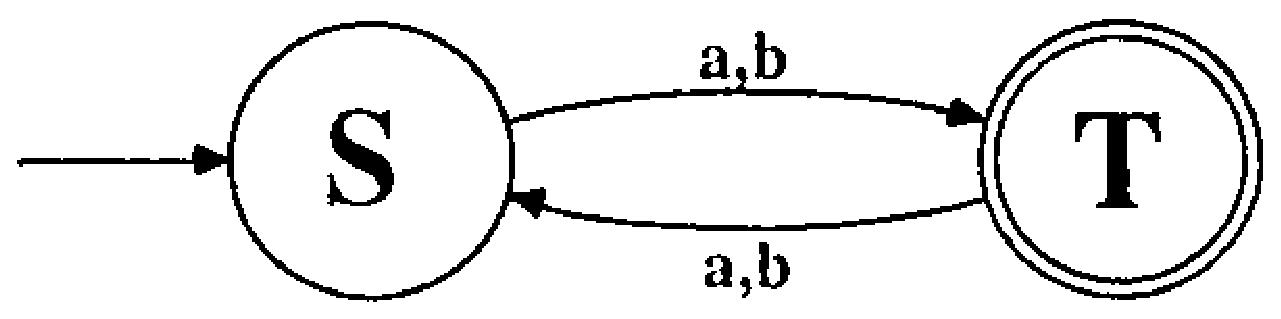
\epsfig{figure=ToFAfigures/fig8-1.eps,width=3in}}
\caption{The automaton discussed in Example 8.10}\label{fig-8.1}
\end{figure}

Lemma \ref{lmm-8.1} showed that a cognitive representation of a finite automaton definable
language can be expressed in an appropriate generative form (via a right-linear
grammar). There are many practical applications in which it is necessary to test
whether certain strings can be generated by a particular grammar. For
unrestricted grammars, the answers to such questions can be far from obvious. In
contrast, the specialized right-linear grammars discussed in this section can
always be transformed into a simple cognitive representation: every right-linear
grammar has a corresponding equivalent NDFA.

% Lemma 8.2
\begin{lmm}\label{lmm-8.2}
Let $\Sigma$ be any alphabet and $G=\langle\Omega,\Sigma,S,P\rangle$ be a
right-linear grammar, then there exists an NDFA $A_G$ (with $\lambda$-transitions)
for which $L(G)=L(A_G)$.

\emph{Proof.} Define $A_G=\langle\Sigma,Q_G,q_{0_G},\delta_G,F_G\rangle$, where
\begin{center}\begin{tabular}{r@{ }l}
$Q_G =$ & $\{\langle z\rangle\ |\ z=\lambda\vee z\in\Omega\vee\exists y\in
		\Sigma^*$ and $\exists B\in\Omega$ \\
& such that $B\rightarrow yz$ is a production in $P\}$ \\
$q_{0_G} =$ & $\{\langle S\rangle\}$ \\
$F_G =$ & $\{\langle\lambda\rangle\}$,
\end{tabular}\end{center}
and $\delta_G$ is comprised of (normal) transitions of the form
\begin{center}\begin{tabular}{r@{ }l}
$\delta_G(\langle w\rangle,\pmb{a}) =$ & $\{\langle x\rangle\ |\ \exists y\in(\Omega
	\cup\Sigma)^*,\exists B\in\Omega\ni w=\pmb{a}x \wedge B\rightarrow yw$ \\
& is a production in $P\}$
\end{tabular}\end{center}
$\delta_G$ also contains some $\lambda$-transitions of the form
\[ \delta_G(\langle B\rangle,\lambda)=\{\langle v\rangle\ |\ B\rightarrow v\text{ is
	a production in }P\} \]
As in the proof of Lemma \ref{lmm-8.1}, there is a one-to-one correspondence between paths
through the machine and derivations in the grammar. Inductive statements will be
the basis from which it will follow that $L(A_G)=L(G)$ (see the exercises).
\end{lmm}

The following example may be helpful in providing a firmer grasp of the
nature of $A_G$.

\subsection*{Example 8.11}

Let $G_1=\langle\{T,S\},\{\pmb{a},\pmb{b}\},S,\{S\rightarrow\pmb{a}S,S\rightarrow
\pmb{b}T,T\rightarrow\pmb{aa}\}\rangle$. Then
\[ A_{G_1}=\langle\{\pmb{a},\pmb{b}\},\{\langle\pmb{a}S\rangle,\langle S\rangle,
	\langle\pmb{b}T\rangle,\langle T\rangle,\langle\pmb{aa}\rangle,\langle
	\pmb{a}\rangle,\langle\lambda\rangle\},\{\langle S\rangle\},\delta_{G_1},
	\{\langle\lambda\rangle\}\rangle, \]
where $\delta_{G_1}$ is given by
\begin{center}\begin{tabular}{r@{ = }l@{$\qquad$}r@{ = }l}
$\delta_{G_1}(\langle S\rangle,\lambda)$ & $\{\langle\pmb{a}S\rangle,\langle
	\pmb{b}T\rangle\}$ & $\delta_{G_1}(\langle T\rangle,\lambda)$ &
	$\{\langle\pmb{aa}\rangle\}$ \\
$\delta_{G_1}(\langle\pmb{a}S\rangle,\pmb{a})$ & $\{\langle S\rangle\}$ &
	$\delta_{G_1}(\langle\pmb{b}T\rangle,\pmb{b})$ & $\{\langle T\rangle\}$ \\
$\delta_{G_1}(\langle\pmb{aa}\rangle,\pmb{a})$ & $\{\langle\pmb{a}\rangle\}$ &
	$\delta_{G_1}(\langle\pmb{a}\rangle,\pmb{a})$ & $\{\langle\lambda\rangle\}$
\end{tabular}\end{center}
and all other transitions are empty [for example, $\delta_{G_1}(\langle S\rangle,
\pmb{a}) = \emptyset$]. This automaton is shown in Figure \ref{fig-8.2}. Note that
$\pmb{abaa}$ is accepted by this machine by visiting the states $\langle S\rangle,\ 
\langle\pmb{a}S\rangle,\ \langle S\rangle,\ \langle\pmb{b}T\rangle,\ \langle T
\rangle,\ \langle\pmb{aa}\rangle,\ \langle\pmb{a}\rangle,\ \langle\lambda\rangle$,
and that the corresponding derivation in $G_1$ is $S\Rightarrow\pmb{a}S
\Rightarrow\pmb{ab}T\Rightarrow\pmb{abaa}$.

% Figure 8.2
\begin{figure}
\centerline{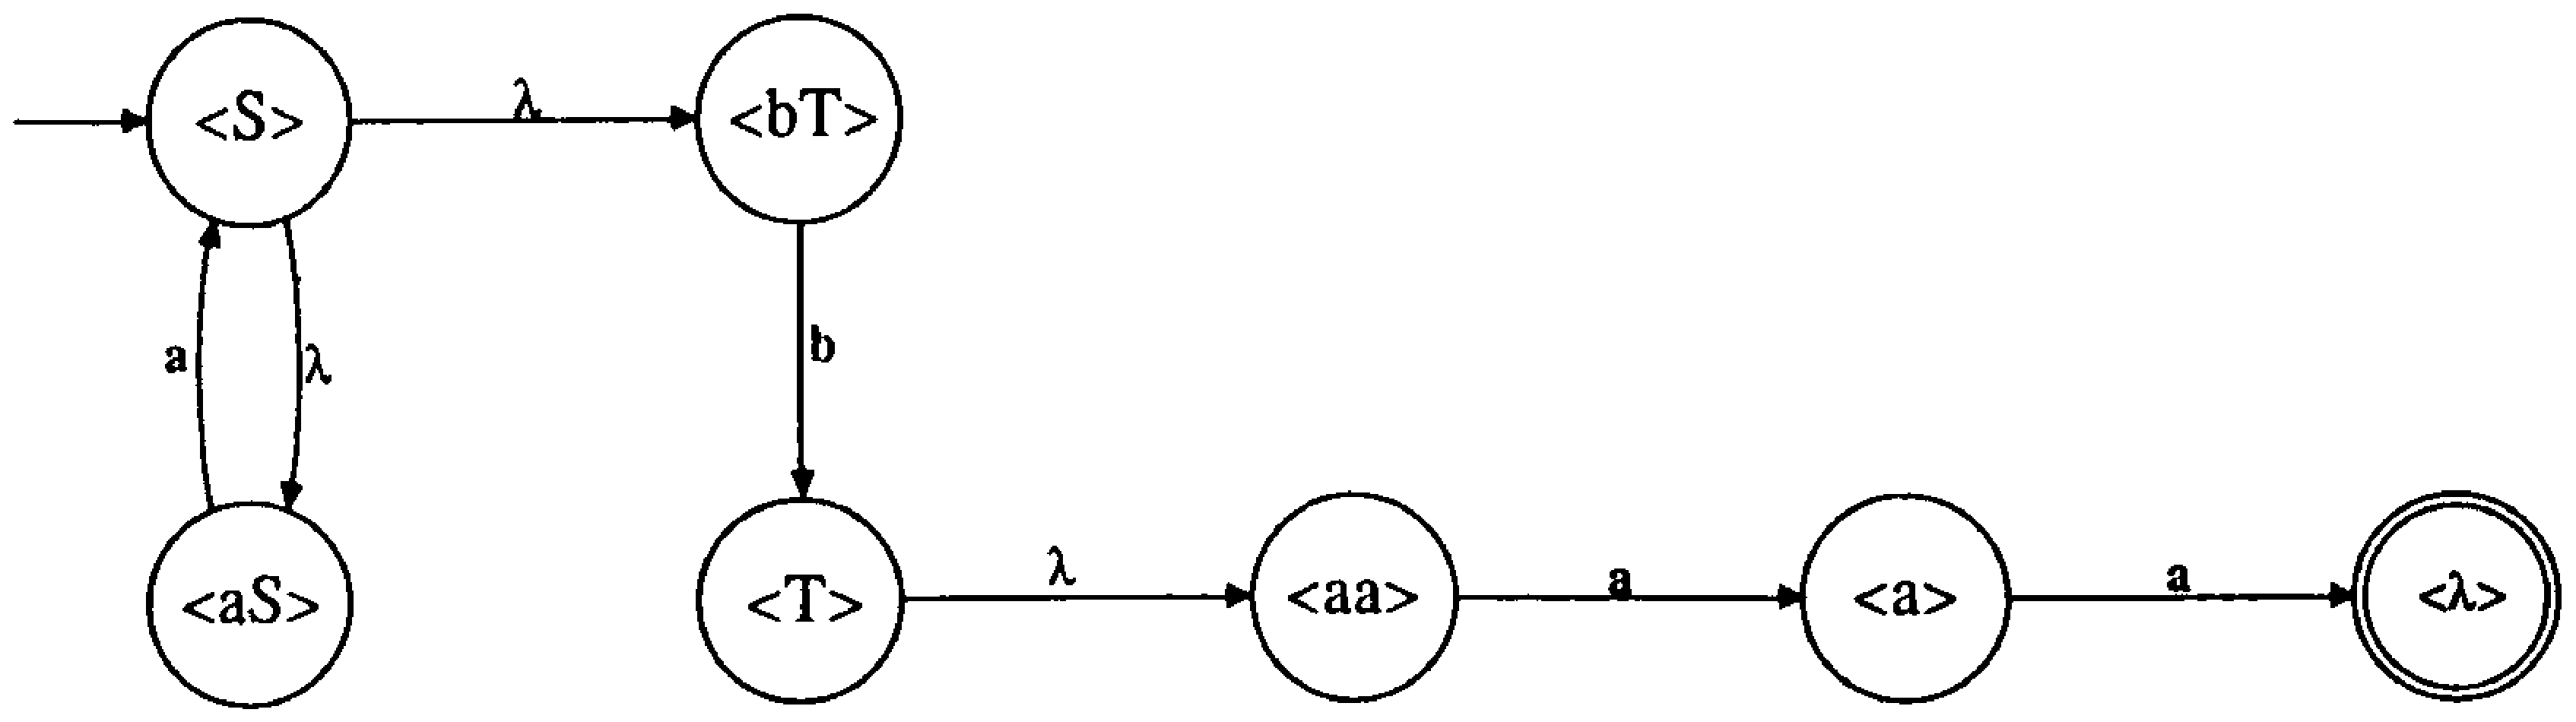
\epsfig{figure=ToFAfigures/fig8-2.eps,width=6.2in}}
\caption{The automaton corresponding to the grammar $G_1$}\label{fig-8.2}
\end{figure}

% Theorem 8.1
\begin{thm}\label{thm-8.1}
Given any alphabet $\Sigma$, $\GSIG = \DSIG$.

\emph{Proof.} Lemma \ref{lmm-8.1} guaranteed that every DFA has a corresponding grammar,
and so $\DSIG\subseteq\GSIG$. By Lemma \ref{lmm-8.2}, every grammar has a corresponding
NDFA, and so $\GSIG\subseteq\WSIG=\DSIG$. Thus $\GSIG=\DSIG$.
\end{thm}

\section{Regular Grammars and Regular Expressions}\label{sec-8.3}

The grammars we have considered so far are called \emph{right} linear because
productions are constrained to have the resulting nonterminal appear to the
right of the terminal symbols. We next consider the class of grammars that
arises by forcing the lone nonterminal to appear to the left of the terminal
symbols.

% Definition 8.11
\begin{dfn}\label{dfn-8.11}\index{language!type $k$}
A \emph{\Index{left-linear grammar}} over an alphabet $\Sigma$ is a quadruple
$G=\langle\Omega,\Sigma,S,P\rangle$, where:

\begin{quote}
$\Omega$ is a (nonempty) set of \emph{nonterminals}. \\
$\Sigma$ is a (nonempty) set of \emph{terminal symbols} (and $\Omega\cap\Sigma =
	\emptyset$). \\
$S$ is the designated \emph{start symbol} (and $S\in\Omega$). \\
$P$ is a set of \emph{productions} of the form $A\rightarrow Bx$, where $A\in\Omega,B
	\in(\Omega\cup\lambda)$, and $x\in\Sigma^*$.
\end{quote}
\end{dfn}
Note that a typical production might now look like $A\rightarrow B\pmb{cd}$,
where the nonterminal $B$ occurs to the left of the terminal string $\pmb{cd}$.

\subsection*{Example 8.12}

Let $G_2=\langle\{A,S\},\{\pmb{a},\pmb{b}\},S,\{S\rightarrow A\pmb{baa},A
\rightarrow A\pmb{a},A\rightarrow \lambda\}\rangle$. Then
\[ L(G_2)=\pmb{a}^*\pmb{baa}=\{\pmb{baa},\pmb{abaa},\pmb{aabaa},\ldots\} =
	L(G_1), \]
and so $G_2 \simeq G_1$ (compare with Example 8.7). Note that there does not
seem to be an obvious way to transform the right-linear grammar $G_1$ discussed
in Example 8.7 into an equivalent left-linear grammar such as $G_2$ (see the
exercises).

As was done for right-linear grammars in the last section, we \emph{could} show
that these left-linear grammars also generate the set of regular languages by
constructing corresponding machines and grammars (see the exercises). However,
we will instead prove that left-linear grammars are equivalent in power to
right-linear grammars by applying known results from previous chapters. The key
to this strategy is the reverse operator $r$ (compare with Example 4.10 and
Exercises 5.20 and 6.36).

% Definition 8.12
\begin{dfn}\label{dfn-8.12}
For an alphabet $\Sigma$, and $x=\pmb{a}_1\pmb{a}_2\cdots\pmb{a}_{n-1}\pmb{a}_n
\in\Sigma^*$; define $x^r=\pmb{a}_n\pmb{a}_{n-1}\cdots\pmb{a}_2\pmb{a}_1$. For a
language $L$ over $\Sigma$, define $L^r=\{x^r\ |\ x\in L\}$. For a grammar $G =
\langle\Omega,\Sigma,S,P\rangle$, define $G^r=\langle\Omega,\Sigma,S,P'\rangle$,
where $P'$ is given by $P'=\{A\rightarrow x^r\ |\ A\rightarrow x$ was a production
in $P\}$.
\end{dfn}

% Lemma 8.3
\begin{lmm}\label{lmm-8.3}
Let $G$ be a right-linear grammar. Then $G^r$ is a left-linear grammar, and
$L(G^r) = L(G)^r$. Similarly, if $G$ is a left-linear grammar, then $G^r$ is a
right-linear grammar, and again $L(G^r) = L(G)^r$.

\emph{Proof.} A straightforward induction on the number of productions used to
produce a given terminal string (see the exercises). It can be shown that $S 
\,\DRightarrow Bx$ by applying $n$ productions from $G$ iff $S\,\DRightarrow x^rB$
by applying $n$ corresponding productions from $G^r$.
\end{lmm}

\subsection*{Example 8.13}

Consider
\[ G_3=\langle\{T,S\},\{\pmb{a},\pmb{b},\pmb{c},\pmb{d}\},S,\{S\rightarrow
	\pmb{ab}S,S\rightarrow\pmb{cd}T,T\rightarrow\pmb{b}T,T\rightarrow
	\pmb{b}\}\rangle. \]
Then
\begin{center}\begin{tabular}{r@{ = }l}
$G_3^r$ & $\langle\{T, S\},\{\pmb{a},\pmb{b},\pmb{c},\pmb{d}\},S,\{S\rightarrow
	S\pmb{ba},S\rightarrow T\pmb{dc},T\rightarrow T\pmb{b},T\rightarrow
	\pmb{b}\}\rangle$, \\
$L(G_3)$ & $(\pmb{ab})^*\pmb{cdbb}^*$, $L(G^r_3)=\pmb{b}^*\pmb{bdc}(\pmb{ba})^*,$
\end{tabular}\end{center}
and
\[ L(G^r_3) = L(G_3)^r\ [\text{and }L(G_3) = L(G^r_3)^r]. \]

% Theorem 8.2
\begin{thm}\label{thm-8.2}
Let $\Sigma$ be an alphabet. Then the class of languages generated by the set of
all left-linear grammars over $\Sigma$ is the same as the class of languages
generated by the set of all right-linear grammars over $\Sigma$.

\emph{Proof.} Let $G$ be a left-linear grammar. $G^r$ is then a right-linear
grammar, and $L(G^r)$ is therefore FAD by Theorem \ref{thm-8.1}. Since \DSIG\ is closed
under the reverse operator $r$ (see Exercise 5.20), $L(G^r)^r$ is also FAD. But,
by Lemma \ref{lmm-8.3}, $L(G^r)^r = L(G)$, and so $L(G)$ is FAD. Hence every left-linear
grammar generates a member of \DSIG\ and therefore (by Lemma \ref{lmm-8.3}) has a corresponding
right-linear grammar.

Conversely, if $L$ is generated by a right-linear grammar, then $L$ is a
language in \DSIG, and so is $L^r$ (as shown by Exercise 5.20 or 6.36). Since
$\DSIG=\GSIG$, there is a right-linear grammar $G$ that generates $L^r$, and
hence $G^r$ is a left-linear grammar that generates $L$ (why?). Thus every
right-linear grammar has a corresponding left-linear grammar.
\end{thm}

% Definition 8.13
\begin{dfn}\label{dfn-8.13}\index{language!type $k$}
A \emph{regular} or \emph{\Index{type 3 grammar}} is a grammar that is either
right-linear or left-linear.
\end{dfn}
Thus, the languages generated by left-linear (and hence regular) grammars are
referred to as type 3 languages. The class of type 3 languages is exactly \GSIG.

% Corollary 8.1
\begin{cor}\label{cor-8.1}
The class of languages generated by regular grammars is equal to \GSIG.

\emph{Proof.} The proof follows immediately from Theorem \ref{thm-8.2}.
\end{cor}

With the correspondences developed between the grammatical descriptors and the
mechanical constructs, it is possible to transform a regular expression into
an equivalent grammar by first transforming the representation of the language
into an automaton (as described in Chapter \ref{ch-6}) and then applying Lemma \ref{lmm-8.1} to the
resulting machine. Conversely, the grammar $G_1$ in Example 8.11 gives rise to
the seven-state NDFA $A_{G_1}$ (using Lemma \ref{lmm-8.2}), which could in turn be used to
generate seven equations in seven unknowns. These could then be solved for a
regular expression representing $L(G_1)$ via Theorems \ref{thm-6.1} and \ref{thm-6.2}. A much more
efficient method, which generates equations directly from the productions
themselves, is outlined in the following theorem.

% Theorem 8.3
\begin{thm}\label{thm-8.3}
Let $G=\langle\{S_1,S_2,\ldots,S_n\},\Sigma,S_1,P\rangle$ be a right-linear
grammar, and for each nonterminal $S_i$ define $X_{s_i}$ to be the set of all
terminal strings that can be derived from $S_i$ by using the productions in $P$.
$X_{S_1}$ then represents $L(G)$, and these sets satisfy the language equations
\[ X_{S_k} = E_k\cup A_{k1}X_{S_1}\cup A_{k2}X_{S_2}\cup\cdots\cup A_{kn}X_{S_n},
	\qquad\text{ for }k = 1,2,\ldots,n \]
where $E_i$ is the union of all terminal strings $x$ that appear in productions
of the form $S_i\rightarrow x$, and $A_{ij}$ is the union of all terminal
strings $x$ that appear in productions of the form $S_i\rightarrow xS_j$.

\emph{Proof.} Since $S_1$ is the start symbol, $X_{S_1}$ is by definition the
set of all words that can be derived from the start symbol, and hence $X_{S_1} =
L(G)$. The relationships between the variables $X_{S_i}$ essentially embody the
relationships enforced by the productions in $P$.
\end{thm}

\subsection*{Example 8.14}

Consider $G_1$ from Example 8.11, in which
\[ G_1 = \langle\{T,S\},\{\pmb{a},\pmb{b}\},S,\{S\rightarrow\pmb{a}S,S\rightarrow
	\pmb{b}T,T\rightarrow\pmb{aa}\}\rangle. \]
The corresponding equations are
\begin{center}\begin{tabular}{r@{ = }l}
$X_S$ & $\emptyset\cup\pmb{a}X_S\cup\pmb{b}X_T$ \\
$X_T$ & $\pmb{aa}\cup\emptyset X_S\cup\emptyset X_T$
\end{tabular}\end{center}
Eliminating $X_T$ via Theorem \ref{thm-6.2} yields $X_S=\pmb{baa}\cup\pmb{a}X_S$. Theorem
\ref{thm-6.1} can be applied to this equation to yield $X_S=L(G_1)=\pmb{a}^*\pmb{baa}$.
Solving these two equations is indeed preferable to appealing the resulting NDFA
from Example 8.11 and solving the corresponding seven equations.

\subsection*{Example 8.15}

Let $\Sigma=\{\pmb{a},\pmb{b},\pmb{c}\}$, and consider the set of all words that
end in $\pmb{b}$ and for which every $\pmb{c}$ is immediately followed by $\pmb{a}$.
This can be succinctly described by the grammar $G=\langle\{S\},\{\pmb{a},
\pmb{b},\pmb{c}\},S,\{S\rightarrow\pmb{a}S,S\rightarrow\pmb{b}S,S\rightarrow
\pmb{ca}S,S\rightarrow\pmb{b}\}\rangle$. The resulting one equation in the
single unknown $X_S$ is $X_S=\pmb{b}\cup(\pmb{a}\cup\pmb{b}\cup\pmb{ca})X_S$,
and Theorem \ref{thm-6.1} can be applied to yield a regular expression for this language;
that is, $X_S=(\pmb{a}\cup\pmb{b}\cup\pmb{ca})^*\pmb{b}$.

Unfortunately, another grammar that generates this same language is
\[ G'=\langle\{S\},\{\pmb{a},\pmb{b},\pmb{c}\},S,\{S\rightarrow\lambda S,S
	\rightarrow\pmb{a}S,S\rightarrow\pmb{b}S,S\rightarrow\pmb{ca}S,S
	\rightarrow\pmb{b}\}\rangle. \]
In this case, however, the resulting one equation in the single unknown $X_S$ is
$X_S=\pmb{b}\cup(\lambda\cup\pmb{a}\cup\pmb{b}\cup\pmb{ca})X_S$, and Theorem \ref{thm-6.1}
explicitly prohibits $\lambda$ from appearing as a coefficient of an unknown.
The equation no longer has a unique solution; other solutions are now possible,
such as $X_S=\Sigma^*$. Nevertheless, the reduction described by Theorem \ref{thm-6.1}
still predicts the correct expression for this language; that is, $X_S=(\lambda
\cup\pmb{a}\cup\pmb{b}\cup\pmb{ca})^*\pmb{b}$. For equations arising from
grammatical constructs, the desired solution will \emph{always} be the minimal
solution predicted by the technique used in Theorem \ref{thm-6.1}. The condition
prohibiting $\lambda$ from appearing in the set $A$ in the equation $X=E\cup AX$
was required to guarantee a unique solution. Regardless of the nature of the set
$A$, $A^*E$ is guaranteed to be a solution, and it will be contained in any
other solution, as restated in Lemma \ref{lmm-8.4}.

% Lemma 8.4
\begin{lmm}\label{lmm-8.4}
Let $E$ and $A$ be any two sets, and consider the language equation $X=E\cup AX$.
$A^*E$ is always a solution for $X$, and any other solution $Y$ must satisfy the
property $A^*E \subseteq Y$.

\emph{Proof.} Follows immediately from Theorem \ref{thm-6.1}.
\end{lmm}

Consider again the grammar
\[ G' = \langle\{S\},\{\pmb{a},\pmb{b},\pmb{c}\},S,\{S\rightarrow\lambda S,S
	\rightarrow\pmb{a}S,S\rightarrow\pmb{b}S,S\rightarrow\pmb{ca}S,S
	\rightarrow\pmb{b}\}\rangle, \]
which generates the language $(\lambda\cup\pmb{a}\cup\pmb{b}\cup\pmb{ca})^*
\pmb{b}$. The corresponding equation was $X=E\cup AX$, where $E=\pmb{b}$, and
$A=(\lambda\cup\pmb{a}\cup\pmb{b}\cup\pmb{ca})$. Note that $E$ represents the
set of terminal strings that can be generated from $S$ using exactly one
production, while $A\cdot E=(\lambda\cup\pmb{a}\cup\pmb{b}\cup\pmb{ca})\pmb{b}$
is the set of all strings that can be generated from $S$ using exactly two
productions. Similarly, $A\cdot A\cdot E$ represents all terminal strings
that can be generated from $S$ using exactly three productions. By induction, it
can be shown that $A^{n-1}\cdot E$ is the set of all strings that can be
generated from S using exactly $n$ productions. From this it follows that the
minimal solution $A^*E$ is indeed the language generated by the grammar.

Clearly, a useless production of the form $S\rightarrow\lambda S$ in a grammar
can simply be removed from the production set without affecting the language
that is generated. In the above example, it was the production $S\rightarrow
\lambda S$ that was responsible for $\lambda$ appearing in the coefficient set
$A$. It is only the \emph{nongenerative} productions, which do not produce any
terminal symbols, that can give rise to a nonunique solution. However, the
removal of productions of the form $V\rightarrow\lambda T$ will require the
addition of other productions when $T$ is a different nonterminal than $V$.
Theorem \ref{thm-9.4}, developed later, will show that these grammars can be transformed
into equivalent grammars that do not contain productions of the form $V
\rightarrow\lambda T$. Theorem \ref{thm-8.4} shows that it is not necessary to perform
such transformations before producing equations that will provide equivalent
regular expressions: the techniques outlined in Theorem \ref{thm-6.2} can indeed be used
to solve systems of equations, even if the coefficients contain the empty word.
Indeed, the minimal solution found in this manner will be the regular expression
sought. This robustness is similar to that found in Theorem \ref{thm-6.3}, which was
stated for deterministic finite automata. Regular expressions for
nondeterministic finite automata can be generated by transforming the NDFA into
a DFA and then applying Theorem \ref{thm-6.3}, but it was seen that it is both possible
and more efficient to apply the method directly to the NDFA without performing
the transformation. The following theorem justifies that a transformation to a
well-behaved grammar is an unnecessary step in the algorithm for finding a
regular expression describing the language generated by a right-linear grammar.

% Lemma 8.5
\begin{lmm}\label{lmm-8.5}
Consider the system of equations in the unknowns $X_1,X_2,\ldots,X_n$ given by
\begin{center}\begin{tabular}{r@{ }c@{ }l}
$X_1$ & $=$ & $E_1\cup A_{11}X_1\cup A_{12}X_2\cup\cdots\cup A_{1(n-1)}X_{n-1}
	\cup A_{1n}X_n$ \\
$X_2$ & $=$ & $E_2\cup A_{21}X_{1}\cup A_{22}X_2\cup\cdots\cup A_{2(n-1)}X_{n-1}
	\cup A_{2n}X_n$ \\
& $\cdot$ \\
& $\cdot$ \\
& $\cdot$ \\
$X_{n-1}$ & $=$ & $E_{n-1}\cup A_{(n-1)1}X_1\cup A_{(n-1)2}X_2\cup\cdots\cup
	A_{(n-1)(n-1)}X_{n-1}\cup A_{(n-1)n}X_n$ \\
$X_n$ & $=$ & $E_n\cup A_{n1}X_1\cup A_{n2}X_2\cup\cdots\cup A_{n(n-1)}X_{n-1}
	\cup A_{nn}X_n$
\end{tabular}\end{center}
\begin{enumerate}[a.]
\item Define $\hat{E}_i = E_i\cup (A_{in}\cdot A^*_{nn}\cdot E_n)$ for all $i =
1,2,\ldots,n-1$ and
\[ \hat{A}_{ij}=A_{ij}\cup(A_{in}\cdot A^*_{nn}\cdot A_{nj})\text{ for all }i,j
	= 1,2,\ldots,n-1. \]
Any solution of the original set of equations will agree with a solution of
the following set of $n-1$ equations in the unknowns $X_1,X_2,\ldots,X_{n-1}$:
\begin{center}\begin{tabular}{r@{ }c@{ }l}
$X_1$ & $=$ & $\hat{E}_1\cup \hat{A}_{11}X_1\cup\hat{A}_{12}X_2\cup\cdots\cup
	\hat{A}_{1(n-1)}X_{n-1}$ \\
$X_2$ & $=$ & $\hat{E}_2\cup \hat{A}_{21}X_{1}\cup\hat{A}_{22}X_2\cup\cdots\cup
	\hat{A}_{2(n-1)}X_{n-1}$ \\
& $\cdot$ \\
& $\cdot$ \\
& $\cdot$ \\
$X_{n-1}$ & $=$ & $\hat{E}_{n-1}\cup \hat{A}_{(n-1)1}X_1\cup\hat{A}_{(n-1)2}X_2
	\cup\cdots\cup\hat{A}_{(n-1)(n-1)}X_{n-1}$
\end{tabular}\end{center}

\item Given a solution to the above $n-1$ equations in (a), that solution can be
used to find a compatible expression for the remaining unknown:
\[ X_n=A^*_{nn}\cdot(E_n\cup A_{n1}X_1\cup A_{n2}X_2\cup\cdots\cup A_{n(n-1)}
	X_{n-1}) \]

\item This system has a unique \emph{minimal} solution in the following sense:
Let $W_1,W_2,\ldots,W_n$ denote the solution found by eliminating variables and
back-substituting as specified in (a) and (b). If $Y_1,Y_2,\ldots,Y_n$ is any
other solution to the original $n$ equations in $n$ unknowns, then $W_1\subseteq
Y_1,W_2\subseteq Y_2,\ldots$, and $W_n\subseteq Y_n$.
\end{enumerate}

\emph{Proof.} This proof is by induction on the number of equations. Lemma \ref{lmm-8.4}
proved the basis step for $n=1$. As in Theorem \ref{thm-6.2}, the inductive step is proved
by considering the last of the $n$ equations,
\[ X_n = (E_n\cup A_{n1}X_1\cup A_{n2}X_2\cup\cdots\cup A_{n(n-1)}X_{n-1})\cup
	A_{nn}X_n \]
This can be thought of as an equation in the one unknown $X_n$ with a coefficient
of $A_{nn}$ for $X_n$, and the remainder of the expression a ``constant'' term
not involving $X_n$.

For a given solution for $X_1$ through $X_{n-1}$ Lemma \ref{lmm-8.4} can therefore be
applied to the above equation in the one unknown $X_n$, with coefficients
\[ E = (E_n\cup A_{n1}X_1\cup A_{n2}X_2\cup\cdots\cup A_{n(n-1)}X_{n-1}) \]
and $A=A_{nn}$ to find a minimal solution for $X_n$ for the corresponding values of
$X_1$ through $X_{n-1}$. This is exactly as given by part (b) above:
\[ X_n=A^*_{nn}\cdot(E_n\cup A_{n1}X_1\cup A_{n2}X_2\cup\cdots\cup A_{n(n-1)}
	X_{n-1}) \]
or
\[ X_n = A^*_{nn}\cdot E_n\cup A^*_{nn}\cdot A_{n1}X_1\cup A^*_{nn}\cdot A_{n2}
	X_2\cup\cdots\cup A^*_{nn}\cdot A_{n(n-1)}X_{n-1}) \]
Specifically, if $X_1$ through $X_{n-1}$ are represented by a minimal solution
$W_1$ through $W_{n-1}$, then Lemma \ref{lmm-8.4} implies that the inclusion of $W_n$,
given by
\[ W_n = A^*_{nn}\cdot E_n\cup A^*_{nn}\cdot A_{n1}W_1\cup A^*_{nn}\cdot A_{n2}
	W_2\cup\cdots\cup A^*_{nn}\cdot A_{n(n-1)}W_{n-1} \]
will yield a minimal solution $W_1$ through $W_n$ of the original $n$ equations
in $n$ unknowns.

The minimal solution for the $n-1$ equations in the unknowns $X_1,X_2,\ldots,
X_{n-1}$, denoted by $W_1$ through $W_{n-1}$ can be found by substituting this
particular solution $W_n$ for $X_n$ in each of the other $n-1$ equations. If the
$k^{th}$ equation is represented by
\[ X_k = E_k\cup A_{k1}X_1\cup A_{k2}X_2\cup\cdots\cup A_{kn}X_n \]
then the substitution will yield
\begin{center}\begin{tabular}{r@{ }l}
$X_k =$ & $E_k\cup A_{k1}X_1\cup A_{k2}X_2\cup\cdots$ \\
& $\cup\ (A_{kn}\cdot(A^*_{nn}\cdot E_n\cup A^*_{nn}\cdot A_{n1}X_1\cup A^*_{nn}
	\cdot A_{n2}X_2\cup\cdots\cup A^*_{nn}\cdot A_{n(n-1)}X_{n-1}))$
\end{tabular}\end{center}
Due to the nature of union and concatenation, no other solution for $X_n$ can
possibly allow a smaller solution for $X_1,X_2,\ldots,X_{n-1}$ to be found.
Specifically, if $Y_n$ is a solution satisfying the $n^{th}$ equation, then Lemma
\ref{lmm-8.4} guarantees that $W_n \subseteq Y_n$, and consequently
\[ X_k = E_k\cup A_{k1}X_1\cup A_{k2}X_2\cup\cdots\cup A_{kn}W_n \subseteq E_k
	\cup A_{k1}X_1\cup A_{k2}X_2\cup\cdots\cup A_{kn}Y_n \]
Thus, the minimal value for each $X_k$ is compatible with the substitution of
$W_n$ defined earlier. Hence, by using the distributive law, the revised
equation becomes
\begin{center}\begin{tabular}{r@{ }l}
$X_k =$ & $E_k\cup A_{k1}X_1\cup A_{k2}X_2\cup\cdots\cup(A_{kn}\cdot A^*_{nn}\cdot
	E_n\cup A_{kn}\cdot A^*_{nn}\cdot A_{n1}X_1$ \\
& $\cup\ A_{kn}\cdot A^*_{nn}\cdot A_{n2}X_2\cup\cdots\cup A_{kn}\cdot A^*_{nn}
	\cdot A_{n(n-1)}X_{n-1})$
\end{tabular}\end{center}
Collecting like terms yields
\begin{center}\begin{tabular}{r@{ }l}
$X_k =$ & $(E_k\cup A_{kn}\cdot A^*_{nn}\cdot E_n)\cup(A_{k1}X_1\cup A_{kn}\cdot
	A^*_{nn}\cdot A_{n1}X_1)$ \\
& $\cup\ (A_{k2}X_2\cup A_{kn}\cdot A^*_{nn}\cdot A_{n2}X_2)\cup\cdots\cup
	(A_{k(n-1)}X_{n-1}\cup A_{kn}\cdot A^*_{nn}\cdot A_{n(n-1)}X_{n-1})$,
\end{tabular}\end{center}
or
\begin{center}\begin{tabular}{r@{ }l}
$X_k =$ & $(E_k\cup A_{kn}\cdot A^*_{nn}\cdot E_n)\cup(A_{k1}\cup A_{kn}\cdot
	A^*_{nn}\cdot A_{n1})X_1$ \\
& $\cup\ (A_{k2}\cup A_{kn}\cdot A^*_{nn}\cdot A_{n2})X_2\cup\cdots\cup(A_{k(n-1
	)}\cup A_{kn}\cdot A^*_{nn}\cdot A_{n(n-1)})X_{n-1}$
\end{tabular}\end{center}
The constant term in this equation is $(E_k\cup A_{kn}\cdot A^*_{nn}\cdot E_n)$,
and the coefficient for $X_j$ is $\hat{A}_{kj} = A_{kj}\cup(A_{kn}\cdot A^*_{nn}
\cdot A_{nj})$, which agrees with the formula given in (a). The substitution of
$X_n$ was shown to yield a minimal set of $n-1$ equations in the unknowns $X_1$
through $X_{n-1}$, and the induction assumption guarantees that the elimination
and back-substitution method yields a minimal solution for $W_1$ through
$W_{n-1}$. Lemma \ref{lmm-8.4} then guarantees that the solution for
\[ W_n = A^*_{nn}\cdot E_n\cup A^*_{nn}\cdot A_{n1}W_1\cup A^*_{nn}\cdot A_{n2}
	W_2\cup\cdots\cup A^*_{nn}\cdot A_{n(n-1)}W_{n-1} \]
is minimal, which completes the minimal solution for the original system of $n$
equations.
\end{lmm}

As with Lemma \ref{lmm-8.4}, the minimal expressions thus generated describe exactly
those terminal strings that can be produced by a right-linear grammar. In an
analogous fashion, left-linear grammars give rise to a set of left-linear
equations, which can be solved as indicated in Theorem \ref{thm-6.4}.

The above discussion describes the transformation of regular grammars into
regular expressions. Generating grammars from regular expressions hinges on
the interpretation of the six building blocks of regular expressions, as
described in Definition \ref{dfn-6.2}. Since \GSIG\ is the same as \DSIG,\ all the closure
properties known about \DSIG\ must also apply to \GSIG, but it can be
instructive to reprove these theorems using grammatical constructions. Such
proofs will also provide guidelines for directly transforming a regular
expression into a grammar without first constructing a corresponding automaton.

% Theorem 8.4
\begin{thm}\label{thm-8.4}
Let $\Sigma$ be an alphabet. Then \GSIG\ is effectively closed under union.

\emph{Proof.} Let $G_1=\langle\Omega_1,\Sigma,S_1,P_1\rangle$ and $G_2=\langle
\Omega_2,\Sigma,S_2,P_2\rangle$ be two right-linear grammars, and without loss
of generality assume that $\Omega_1\cap\Omega_2=\emptyset$. Choose a new
nonterminal $Z$ such that $Z \notin \Omega_1\cup\Omega_2$, and consider the new
grammar $G^{\cup}$ defined by $G^{\cup}=\langle\Omega_1\cup\Omega_2\cup\{Z\},
\Sigma,Z,P_1\cup P_2\cup\{Z\rightarrow S_1,Z\rightarrow S_2\}\rangle$. It is
straightforward to show that $L(G^{\cup})=L(G_1)\cup L(G_2)$ (see the exercises).
From the start symbol $Z$ there are only two productions that can be applied; if
$Z\rightarrow S_1$ is chosen, then the derivation will have to continue with
productions from $P_1$ and produce a word from $L(G_1)$ (why can't productions
from $P_2$ be applied?). Similarly, if $Z\rightarrow S_2$ is chosen instead, the
only result can be a word from $L(G_2)$.
\end{thm}

In an analogous fashion, effective closure of \GSIG\ can be demonstrated for the
operators Kleene closure and concatenation. The proof for Kleene closure is
outlined below. The construction for concatenation is left for the exercises;
the technique is illustrated in Example 8.18.

% Theorem 8.5
\begin{thm}\label{thm-8.5}
Let $\Sigma$ be an alphabet. Then \GSIG\ is effectively closed under
\Index{Kleene closure}.

\emph{Proof.} Let $G=\langle\Omega,\Sigma,S,P\rangle$ be a right-linear grammar.
Choose a new nonterminal $Z$ such that $Z \notin \Omega$, and consider the new
grammar $G_*$ defined by
\[ G_* = \langle\Omega\cup\{Z\},\Sigma,Z,P_*\rangle, \]
where
\begin{center}\begin{tabular}{r@{ }l}
$P_* =$ & $\langle\{Z\rightarrow\lambda,Z\rightarrow S\}$ \\
& $\cup\{A\rightarrow xB\ |\ (x\in\Sigma^*)\wedge(A,B\in\Omega)\wedge(A\rightarrow
	xB\in P)\}$ \\
& $\cup\{A\rightarrow xZ\ |\ (x\in\Sigma^*)\wedge(A\in\Omega)\wedge(A\rightarrow x
	\in P)\}\rangle$.
\end{tabular}\end{center}
That is, all productions in $P$ that end in a nonterminal are retained, while
all other productions in $P$ are appended with the new symbol $Z$, and the two
new productions $Z\rightarrow\lambda$ and $Z\rightarrow S$ are added. A
straightforward induction argument will show that the derivations that use $n$
applications of productions of the form $A\rightarrow xZ$ generate exactly the
words in $L(G)^n$. Consequently, $L(G_*) = L(G)^*$.
\end{thm}

% Theorem 8.6
\begin{thm}\label{thm-8.6}
Let $\Sigma$ be an alphabet. Then \GSIG\ is effectively closed under
concatenation.

\emph{Proof.} See the exercises.
\end{thm}

% Corollary 8.2
\begin{cor}\label{cor-8.2}
Every regular expression has a corresponding right-linear grammar.

\emph{Proof.} While this follows immediately from the fact that $\GSIG=\DSIG$
and Theorem \ref{thm-6.1}, the previous theorems outline an effective procedure for
transforming a regular expression into a right-linear grammar. This can be
proved by induction on the number of operators in the regular expression. The
basis step consists of the observation that expressions with zero operators,
which must be of the form $\emptyset,\ \lambda$, or $\pmb{a}$, can be represented
by the right-linear grammars $\langle\{S\},\Sigma,S,\{S\rightarrow S\}\rangle$,
$\langle\{S\},\Sigma,S,\{S\rightarrow\lambda\}\rangle$, and $\langle\{S\},\Sigma,
S,\{S\rightarrow\pmb{a}\}\rangle$, respectively.

To prove the inductive step, choose an arbitrary regular expression $R$ with
$m+1$ operators, and identify the outermost operator. $R$ must be of the form
$R_1\cup R_2$ or $R_1\cdot R_2$ or $R^*_1$, where $R_1$ (and $R_2$) have $m$ or
fewer operators. By the induction hypothesis, $R_1$ (and $R_2$) can be
represented as right-linear grammars, and therefore by Theorem \ref{thm-8.4}, \ref{thm-8.5}, or \ref{thm-8.6},
$R$ can also be represented by a right-linear grammar. Any regular expression
can thus be methodically transformed into an equivalent right-linear grammar.
\end{cor}

\subsection*{Example 8.16}

Let $\Sigma=\{\pmb{a},\pmb{b},\pmb{c}\}$, and consider the regular expression
$(\pmb{a}\cup\pmb{b})$. The grammars $G_1=\langle\{R\},\{\pmb{a},\pmb{b},\pmb{c}
\},R,\{R\rightarrow\pmb{a}\}\rangle$ and $G_2=\langle\{T\},\{\pmb{a},\pmb{b},
\pmb{c}\},T,\{T\rightarrow\pmb{b}\}\rangle$ can be combined as suggested in
Theorem \ref{thm-8.4} (with $A$ playing the role of $Z$) to form $G=\langle\{T,R,A\},\{
\pmb{a},\pmb{b},\pmb{c}\},A,\{A\rightarrow R,A\rightarrow T,R\rightarrow\pmb{a},
T\rightarrow\pmb{b}\}\rangle$.

\subsection*{Example 8.17}

Consider the regular expression $(\pmb{a}\cup\pmb{b})^*$. The grammar
\[ G=\langle\{T,R,A\},\{\pmb{a},\pmb{b},\pmb{c}\},A,\{A\rightarrow R,A
	\rightarrow T,R\rightarrow\pmb{a},T\rightarrow\pmb{b}\}\rangle \]
from Example 8.16 can be modified as suggested in Theorem \ref{thm-8.5} to form
\[ G_* = \langle\{T,R,A,Z\},\{\pmb{a},\pmb{b},\pmb{c}\},Z,\{Z\rightarrow\lambda,
	Z\rightarrow A,A\rightarrow R,A\rightarrow T,R\rightarrow\pmb{a}Z,T
	\rightarrow\pmb{b}Z\}\rangle. \]
$G_*$ generates $(\pmb{a}\cup\pmb{b})^*$.

\subsection*{Example 8.18}

Consider the regular expression $(\pmb{a}\cup\pmb{b})^*\pmb{c}$. The grammars
\[ G_* = \langle\{T,R,A,Z\},\{\pmb{a},\pmb{b},\pmb{c}\},Z,\{Z\rightarrow\lambda,
	Z\rightarrow A,A\rightarrow R,A\rightarrow T,R\rightarrow\pmb{a}Z,T
	\rightarrow\pmb{b}Z\}\rangle. \]
and
\[ G_3 = \langle\{V\},\{\pmb{a},\pmb{b},\pmb{c}\},V,\{V\rightarrow\pmb{c}\}
	\rangle \]
can be combined with modified productions to form
\begin{center}\begin{tabular}{r@{ }l}
$G' =$ & $\langle\{T,R,A,Z,V,S\},\{\pmb{a},\pmb{b},\pmb{c}\},S,$ \\
& $\{S\rightarrow Z,Z\rightarrow \lambda V,Z\rightarrow A,A\rightarrow R,A
	\rightarrow T,R\rightarrow\pmb{a}Z,T\rightarrow\pmb{b}Z,V\rightarrow
	\pmb{c}\}\rangle$.
\end{tabular}\end{center}
$G'$ generates $(\pmb{a}\cup\pmb{b})^*\pmb{c}$.

The previous examples illustrate the manner in which regular expressions can
be systematically translated into right-linear grammars. Constructions
corresponding to those given in Theorems \ref{thm-8.4}, \ref{thm-8.5}, and \ref{thm-8.6} can similarly be
found for left-linear grammars (see the exercises).

\emph{Normal forms} for grammars are quite useful in many contexts. A standard
representation can be especially useful in proving theorems about grammars. For
example, the construction given in Lemma \ref{lmm-8.2} would have been more concise and
easier to investigate if complex productions such as $S\rightarrow\pmb{bcaa}T$
could be avoided. Indeed, if all productions in the grammar $G$ had been of the
form $A\rightarrow\pmb{a}B$ or $A\rightarrow\lambda$, both the state set and the
state transition function of $A_G$ could have been defined more easily. Other
constructions and proofs may also be able to make use of the simpler types of
productions in grammars that conform to such normal forms. The following theorem
guarantees that a given right-linear grammar has a corresponding equivalent
grammar containing only productions that conform to the above standard.

% Theorem 8.7
\begin{thm}\label{thm-8.7}
Every right-linear grammar $G$ has an equivalent right-linear grammar $G^1$ in
which all productions are of the form $A\rightarrow\pmb{a}B$ or $A\rightarrow
\lambda$.

\emph{Proof.} Let $G$ be a right-linear grammar. By Lemma \ref{lmm-8.2}, there exists an
NDFA $A_G$ that is equivalent to $G$. From Chapter \ref{ch-4}, $A^d_G$ is an equivalent
deterministic finite automaton, and Lemma \ref{lmm-8.1} can be applied to $A^d_G$ to form
an equivalent right-linear grammar. By the construction given in Lemma \ref{lmm-8.1}, all
the productions in this grammar are indeed of the form $A\rightarrow\pmb{a}B$ or
$A\rightarrow\lambda$.
\end{thm}

Note that the proof given is a constructive proof: rather than simply arguing
the existence of such a grammar, a method for obtaining $G^1$ is outlined. The
above theorem could have been proved without relying on automata constructs.
Basically, ``long'' productions like $T\rightarrow\pmb{abc}R$ would be replaced
by a series of productions involving newly introduced nonterminals, for example,
$T\rightarrow\pmb{a}X,X\rightarrow\pmb{b}Y,Y\rightarrow\pmb{c}R$. Similarly, a
production like $T\rightarrow\pmb{aa}$ might be replaced by the sequence $T
\rightarrow\pmb{a}B,B\rightarrow\pmb{a}C,C\rightarrow\lambda$. If the existence
of such a normal form had been available for the proof of Lemma \ref{lmm-8.2}, the
construction of $A_G$ could have been simplified and the complexity of the proof
drastically curtailed. Indeed, the resulting machine would have contained no
$\lambda$-moves. Only one state per nonterminal would have been necessary, with
final states corresponding to nonterminals that had productions of the form $A
\rightarrow \lambda$. Productions of the form $A\rightarrow\pmb{a}B$ would imply
that $B\in\delta(A,\pmb{a})$.

\subsection*{Example 8.19}

$G = \langle\{S,T,B,C\},\{\pmb{a},\pmb{b}\},S,\{S\rightarrow\pmb{a}S,S
\rightarrow\pmb{b}T,T\rightarrow\pmb{a}B,B\rightarrow\pmb{a}C,C\rightarrow
\lambda\}\rangle$ can be represented by the NDFA shown in Figure \ref{fig-8.3}.

% Figure 8.3
\begin{figure}
\centerline{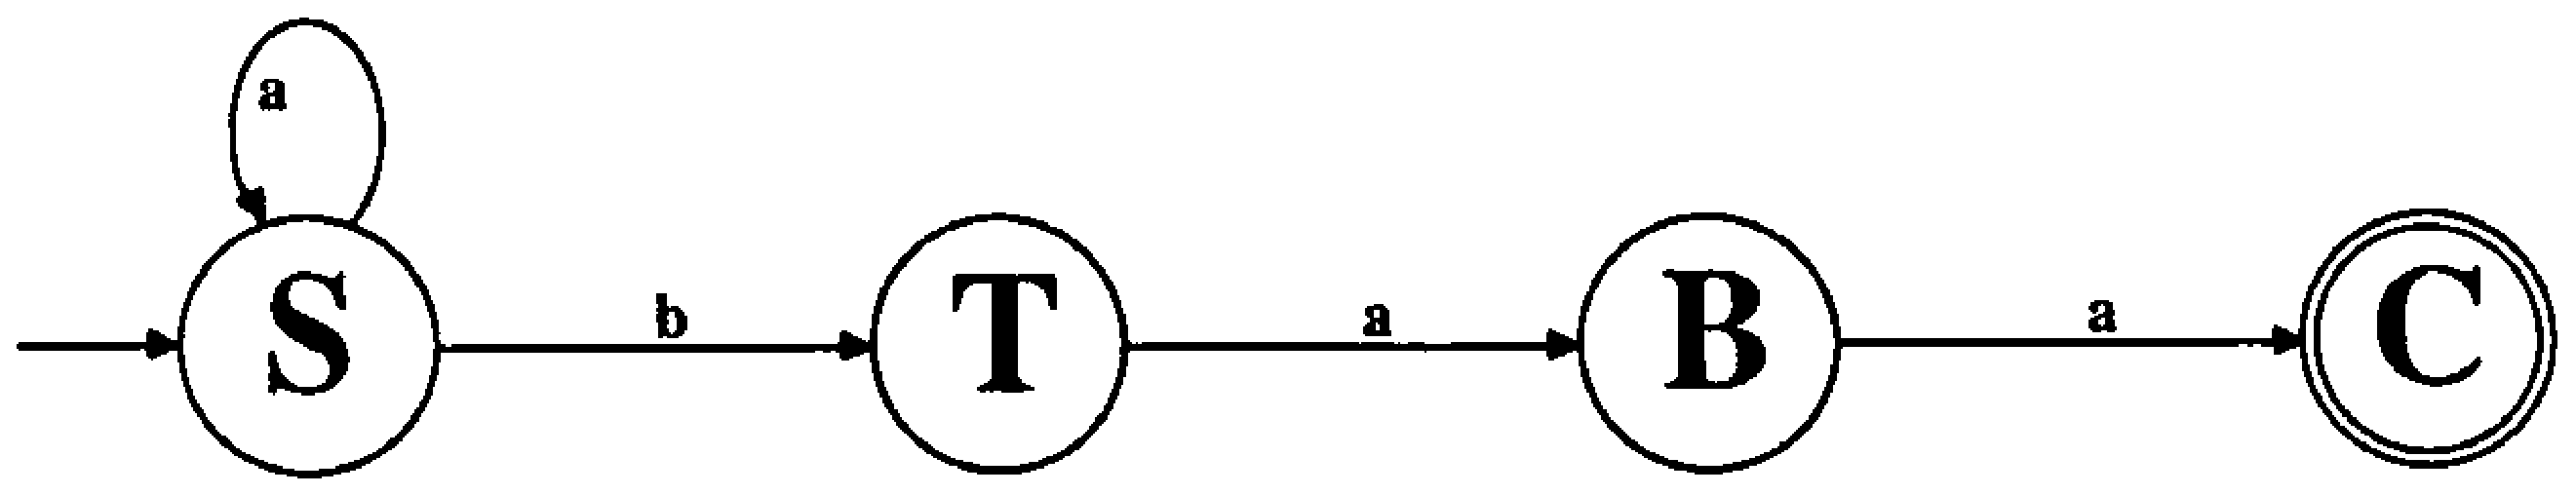
\epsfig{figure=ToFAfigures/fig8-3.eps,width=5.2in}}
\caption{An automaton corresponding to a grammar in normal form}\label{fig-8.3}
\end{figure}

In practice, given an arbitrary right-linear grammar $G$, the work associated
with finding the complex machine defined in Lemma \ref{lmm-8.2} has simply been replaced
by the effort needed to transform $G$ into the appropriate normal form.
Nevertheless, the guarantee that regular languages have grammars that conform to
the above normal form is useful in many proofs, as illustrated above and in
Theorem \ref{thm-8.8} below.

As with context-free and context-sensitive languages, the contracting
productions can be limited to $Z\rightarrow\lambda$, where $Z$ is the start
symbol. This is only necessary if $\lambda\in L$; if $\lambda\notin L$, there
need be no contracting productions at all. We wish to show how to produce a
right-linear grammar with no more than one contracting production. By relying on the
existence of the normal form described in Theorem \ref{thm-8.7}, this can be done without
dealing with right-linear grammars in their full generality.

% Theorem 8.8
\begin{thm}\label{thm-8.8}
Every right-linear grammar $G$ has an equivalent right-linear grammar $G^0$ in
which the start symbol $Z$ never appears on the right in any production, and the
only length-contracting production that may appear is $Z\rightarrow\lambda$.
Furthermore, all other productions are of the form $A\rightarrow\pmb{a}B$ or $A
\rightarrow\pmb{a}$.

\emph{Proof.} Let $G = \langle\Omega,\Sigma,S,P\rangle$ be a right-linear
grammar. Without loss of generality, assume that $G$ is of the form specified by
Theorem \ref{thm-8.7}. (If $G$ were not of the proper form, Theorem \ref{thm-8.7} guarantees that an
equivalent grammar that is in the proper form could be found and used in place
of $G$.) Choose a new nonterminal $Z$ such that $Z\notin\Omega$, and consider
the new grammar $G^0$ defined by $G^0 = \langle\Omega\cup\{Z\},\Sigma,Z,P^0
\rangle$, where $P^0$ contains $Z\rightarrow S$, and all productions from $P$
of the form $A\rightarrow xB$, where $x\in\Sigma^*$ and $A,B \in\Omega$. $P^0$
also contains the productions in the set $\{A\rightarrow\pmb{a}\ |\ (\exists B\in
\Omega)(A\rightarrow\pmb{a}B\in P \wedge B\rightarrow\lambda\in P)\}$. Finally,
if $S\rightarrow\lambda$ was a production in $P$, then $Z\rightarrow\lambda$ is
included in $P^0$. Note that no other productions of the form $B\rightarrow
\lambda$ are part of $P^0$. Other productions have been added to compensate for
this loss. Derivations using the productions in $P^0$ typically start with $Z
\rightarrow S$, then proceed with productions of the form $A\rightarrow xB$, and
terminate with one production of the form $A\rightarrow\pmb{a}$. The
corresponding derivation in the original grammar $G$ would be very similar, but
would start with the old start symbol $S$ and therefore avoid the $Z\rightarrow
S$ application used in $G^0$. The productions of the form $A\rightarrow xB$ are
common to both grammars, and the final step in $G^0$ that uses $A\rightarrow
\pmb{a}$ would be handled by two productions in $G$: $A\rightarrow\pmb{a}B$ and
$B\rightarrow\lambda$. An induction argument on the number of productions in a
derivation will show that every derivation from $G^0$ has a corresponding
derivation in $G$ that produces the same terminal string, and vice versa. Thus,
$L(G^0)=L(G)$, which justifies that $G^0$ is equivalent to $G$. $G^0$ was
constructed to conform to the conditions specified by the theorem, and thus the
proof is complete.
\end{thm}

% Corollary 8.3
\begin{cor}\label{cor-8.3}\index{hierarchy!of grammars}
Every type 3 language is also a type 2 language.

\emph{Proof.} Let $L$ be a type 3 language. Then there exists a right-linear
grammar $G$ that generates $L$. By Theorem \ref{thm-8.8}, there is an equivalent
right-linear grammar $G^0$ that satisfies the definition of a context-free
grammar. Thus, $L$ is context free.
\end{cor}

Section \ref{sec-8.1} explored several generalizations of the definition of a regular
grammar, and, unlike the generalization from DFAs to NDFAs, new and larger
classes of languages result from these generalizations. These new types of
grammars will be explored in the following chapters, and the corresponding
generalized machines will be developed.

\section*{Exercises}

\begin{enumerate}[{8.}1. ]
\item Can strings like $\pmb{ab}BA\pmb{d}B\pmb{c}$ (where $B$ and $A$ are nonterminals)
ever be derived from the start symbol $S$ in a right-linear grammar? Explain.

\item Given $A$ and $G_A$ as defined in Lemma \ref{lmm-8.1}, let $P(n)$ be the statement
that $(\forall x\in\Sigma^n)(\exists j\in\NN)$ [if $t_0\DRightarrow xt_j$, then
$\DBAR_A(t_0,x)=t_j$]. Prove that $P(n)$ is true for all $n\in\NN$.

\item Give regular expressions that describe the language generated by:
\begin{enumerate}
\item $G_4 = \langle\{S,A,B,C,V,W,X\},\{\pmb{a},\pmb{b},\pmb{c}\},S,\{S
	\rightarrow\pmb{ab}A|\pmb{bb}B|\pmb{cc}V,A\rightarrow\pmb{b}C|\pmb{c}X,
	B\rightarrow\pmb{ab},C\rightarrow\lambda|\pmb{c}S,V\rightarrow\pmb{a}V|
	\pmb{c}X,W\rightarrow\pmb{aa}|\pmb{a}W,X\rightarrow\pmb{b}V|\pmb{aa}X\}
	\rangle$
\item $G_5 = \langle\{S_0,S_1,S_2\},\{\pmb{0},\pmb{1}\},S_0,\{S_0\rightarrow
	\lambda|\pmb{0}S_2|\pmb{1}S_1,S_1\rightarrow\pmb{0}S_1|\pmb{1}S_2,S_2
	\rightarrow\pmb{0}S_2|\pmb{1}S_0\}\rangle$
\item $G_6 = \langle\{T,Z\},\{\pmb{a},\pmb{b}\},Z,\{Z\rightarrow\pmb{a}Z,Z
	\rightarrow\pmb{b}T,T\rightarrow\pmb{a}Z\}\rangle$
\item $G_7 = \langle\{S,B,C\},\{\pmb{a},\pmb{b},\pmb{c}\},S,\{S\rightarrow
	\pmb{a}S|\pmb{ab}B|\pmb{c}C,B\rightarrow\pmb{ab}B|\lambda,C\rightarrow
	\pmb{c}C|\pmb{ca}\}\rangle$
\end{enumerate}

\item Use the inductive fact proved in Exercise 8.2 to formally prove Lemma
\ref{lmm-8.1}.

\item Draw the automata corresponding to the grammars given in Exercise 8.3.

\item Give, if possible, right-linear grammars that will generate:
\begin{enumerate}
\item All words in $\{\pmb{a},\pmb{b},\pmb{c}\}^*$ that do \emph{not} contain
	two consecutive $\pmb{b}$s.
\item All words in $\{\pmb{a},\pmb{b},\pmb{c}\}^*$ that \emph{do} contain two
	consecutive $\pmb{b}$s.
\item All words in $\{\pmb{a},\pmb{b},\pmb{c}\}^*$ that have the same number of
	$\pmb{a}$s as $\pmb{b}$s.
\item All words in $\{\pmb{a},\pmb{b},\pmb{c}\}^*$ that have an even number of
	$\pmb{a}$s.
\item All words in $\{\pmb{a},\pmb{b},\pmb{c}\}^*$ that do \emph{not} end in the
	letter $\pmb{b}$.
\item All words in $\{\pmb{a},\pmb{b},\pmb{c}\}^*$ that do \emph{not} contain
	any $\pmb{c}$s.
\end{enumerate}

\item Give left-linear grammars that will generate the languages described in
Exercise 8.6.

\item Complete the inductive portion of the proof of Theorem \ref{thm-8.8}.

\item Complete the inductive portion of the proof of Theorem \ref{thm-8.5}.

\item Use the more efficient algorithm indicated in Theorem \ref{thm-8.3} to find
regular expressions to describe $L(G_5),\ L(G_6)$, and $L(G_7)$ in Exercise 8.3.

\item \begin{enumerate}
\item Restate Theorem \ref{thm-8.3} so that it generates valid language equations
	for left-linear grammars.
\item Restate Lemmas \ref{lmm-8.4} and \ref{lmm-8.5} for these new types of equations.
\item Use your new methods to find a regular expression for $L(G_2)$ in Example
	8.12.
\end{enumerate}

\item Consider the grammar $Q=\langle\{I,F\},\{\pmb{0},\pmb{1},\pmb{.}\},I,\{
I\rightarrow\pmb{0}I|\pmb{1}I|\pmb{0.}F|\pmb{1.}F,F\rightarrow\lambda|\pmb{0}F|
\pmb{1}F\}\rangle$. $L(Q)$ generates the set of all (terminating) binary numbers
including {\bf 101.11}, {\bf 011.}, {\bf 10.0}, {\bf 0.010}, and so on.
\begin{enumerate}
\item Find the corresponding NDFA for this grammar.
\item Write the right-linear equations corresponding to this grammar.
\item Solve the equations found in part (b) for both unknowns.
\end{enumerate}

\item Find right-linear grammars for:
\begin{enumerate}
\item $(\pmb{a}\cup\pmb{b})\pmb{c}^*(\pmb{d}\cup(\pmb{ab})^*)$
\item $(\pmb{a}\cup\pmb{b})^*\pmb{a}(\pmb{a}\cup\pmb{b})^*$
\end{enumerate}

\item Find left-linear grammars for:
\begin{enumerate}
\item $(\pmb{a}\cup\pmb{b})\pmb{c}^*(\pmb{d}\cup(\pmb{ab})^*)$
\item $(\pmb{a}\cup\pmb{b})^*\pmb{a}(\pmb{a}\cup\pmb{b})^*$
\end{enumerate}

\item \begin{enumerate}
\item Describe an \emph{efficient} algorithm that will convert a right-linear
grammar into a left-linear grammar.
\item Apply your algorithm to
\begin{center}\begin{tabular}{r@{ }l}
$G_4 =$ & $\langle\{S,A,B,C,V,W,X\},\{\pmb{a},\pmb{b},\pmb{c}\},S,\{S\rightarrow
	\pmb{ab}A|\pmb{bb}B|\pmb{cc}V,A\rightarrow\pmb{b}C|\pmb{c}X,B\rightarrow
	\pmb{ab}$, \\
& $C\rightarrow\lambda|\pmb{c}S,V\rightarrow\pmb{a}V|\pmb{c}X,W\rightarrow
	\pmb{aa}|\pmb{a}W,X\rightarrow\pmb{b}V|\pmb{aa}X\}\rangle$
\end{tabular}\end{center}
\end{enumerate}

\item Describe an algorithm that will convert a given regular grammar $G$ into
another regular grammar $G'$ that generates the complement of $L(G)$.

\item Without appealing to the tricks used in Chapter \ref{ch-12}, outline an algorithm that
will determine whether the language generated by a given regular grammar $G$ is
empty.

\item Without appealing to the tricks used in Chapter \ref{ch-12}, outline an algorithm that
will determine whether the language generated by a given regular grammar $G$ is
infinite.

\item Without appealing to the tricks used in Chapter \ref{ch-12}, outline an algorithm that
will determine whether two right-linear grammars $G_1$ and $G_2$ generate the
same language.

\item Consider the grammar
\[ H = \langle\{A,B,S\},\{\pmb{a},\pmb{b},\pmb{c}\},S,\{S\rightarrow\pmb{a}SB
	\pmb{c},S\rightarrow\lambda,SB\rightarrow\pmb{b}S,\pmb{c}B\rightarrow
	B\pmb{c}\}\rangle \]
Determine $L(H)$.

\item What is wrong with proving that \GSIG\ is closed under concatenation by
using the following construction? Let $G_1 = \langle\Omega_I,\Sigma,S_1,P_1
\rangle$ and $G_2 = \langle\Omega_2,\Sigma,S_2,P_2\rangle$ be two right-linear
grammars, and, without loss of generality, assume that $\Omega_1\cap\Omega_2 =
\emptyset$. Choose a new nonterminal $Z$ such that $Z\notin\Omega_1\cup\Omega_2$,
and define a new grammar $G^\bullet = \langle\Omega_1\cup\Omega_2\cup\{Z\},\Sigma,Z,
P_1\cup P_2\cup\{Z\rightarrow S_1\cdot S_2\}\rangle$. \emph{Note:} It \emph{is}
straightforward to show that $L(G^\bullet)=L(G_1)\cdot L(G_2)$ (see Chapter \ref{ch-9}).

\item Prove that \GSIG\ is closed under concatenation by:
\begin{enumerate}
\item Constructing a new grammar $G^\bullet$ with the property that $L(G^\bullet)=L(G_1)
\cdot L(G_2)$.
\item Proving that $L(G^\bullet)=L(G_1)\cdot L(G_2)$.
\end{enumerate}

\item Use the constructs presented in this chapter to solve the following
problem from Chapter \ref{ch-4}: Given a nondeterministic finite automaton $A$
\emph{without} $\lambda$-transitions, show that it is possible to construct a
nondeterministic finite automaton \emph{with} $\lambda$-transitions $A'$ with
the properties (1) $A'$ has exactly \emph{one} start state and exactly \emph{one}
final state, and (2) $L(A')=L(A)$.

\item Complete the proof of Lemma \ref{lmm-8.2} by:
\begin{enumerate}
\item Defining an appropriate inductive statement.
\item Proving the statement defined in part (a).
\end{enumerate}

\item Complete the proof of Lemma \ref{lmm-8.3} by:
\begin{enumerate}
\item Defining an appropriate inductive statement.
\item Proving the statement defined in part (a).
\end{enumerate}

\item Fill in the details in the second half of the proof of Theorem \ref{thm-8.2} by
providing reasons for each of the assertions that were made.

\item \begin{enumerate}
\item Refer to Example 8.7 and use induction to formally prove that $L(G_1) =
\{\pmb{a}^n\pmb{baa}|n\in\NN\}$.
\item Refer to Example 8.9 and use induction to formally prove that $L(G_8) =
\{\pmb{a}^n\pmb{baa}|n\in\NN\}$.
\end{enumerate}

\item Notice that regular grammars are defined to have production sets that
contain \emph{only} right-linear-type productions or \emph{only}
left-linear-type productions. Consider the following grammar $C$, which contains
both types of productions:
\[ C = \langle\{S,A,B\},\{\pmb{0},\pmb{1}\},S,\{S\rightarrow\pmb{0}A|\pmb{1}B|
	\pmb{0}|\pmb{1}|\lambda,A\rightarrow S\pmb{0},B\rightarrow S\pmb{1}\}\rangle. \]
Note that $S\Rightarrow\pmb{0}A\Rightarrow\pmb{0}S\pmb{0}\Rightarrow\pmb{01}B
\pmb{0}\Rightarrow\pmb{01}S\pmb{10}\Rightarrow\pmb{0110}$.
\begin{enumerate}
\item Find $L(C)$.
\item Is $L(C)$ FAD?
\item Should the definition of regular grammars be expanded to include grammars
like this one? Explain.
\end{enumerate}

\item \begin{enumerate}
\item Why was it important to assume that $\Omega_1\cap\Omega_2=\emptyset$ in
the proof of Theorem \ref{thm-8.4}? Give an example.
\item Why was it \emph{possible} to assume that $\Omega_1\cap\Omega_2=\emptyset$ in the
proof of Theorem \ref{thm-8.4}? Give a justification.
\end{enumerate}

\item Consider the NDFA $A_G$ defined in Lemma \ref{lmm-8.2}. If $A_G$ is disconnected,
what does this say about the grammar $G$?

\item Apply Lemma \ref{lmm-8.1} to the automata in Figure \ref{fig-8.4}.

\item \begin{enumerate}
\item Restate Lemma \ref{lmm-8.1} so that it directly applies to NDFAs.
\item Prove this new lemma.
\item Assume $\Sigma=\{\pmb{a},\pmb{b},\pmb{c}\}$ and apply this new lemma to
the automata in Figure \ref{fig-8.5}.
\end{enumerate}

% Figure 8.4
\begin{figure}
\centerline{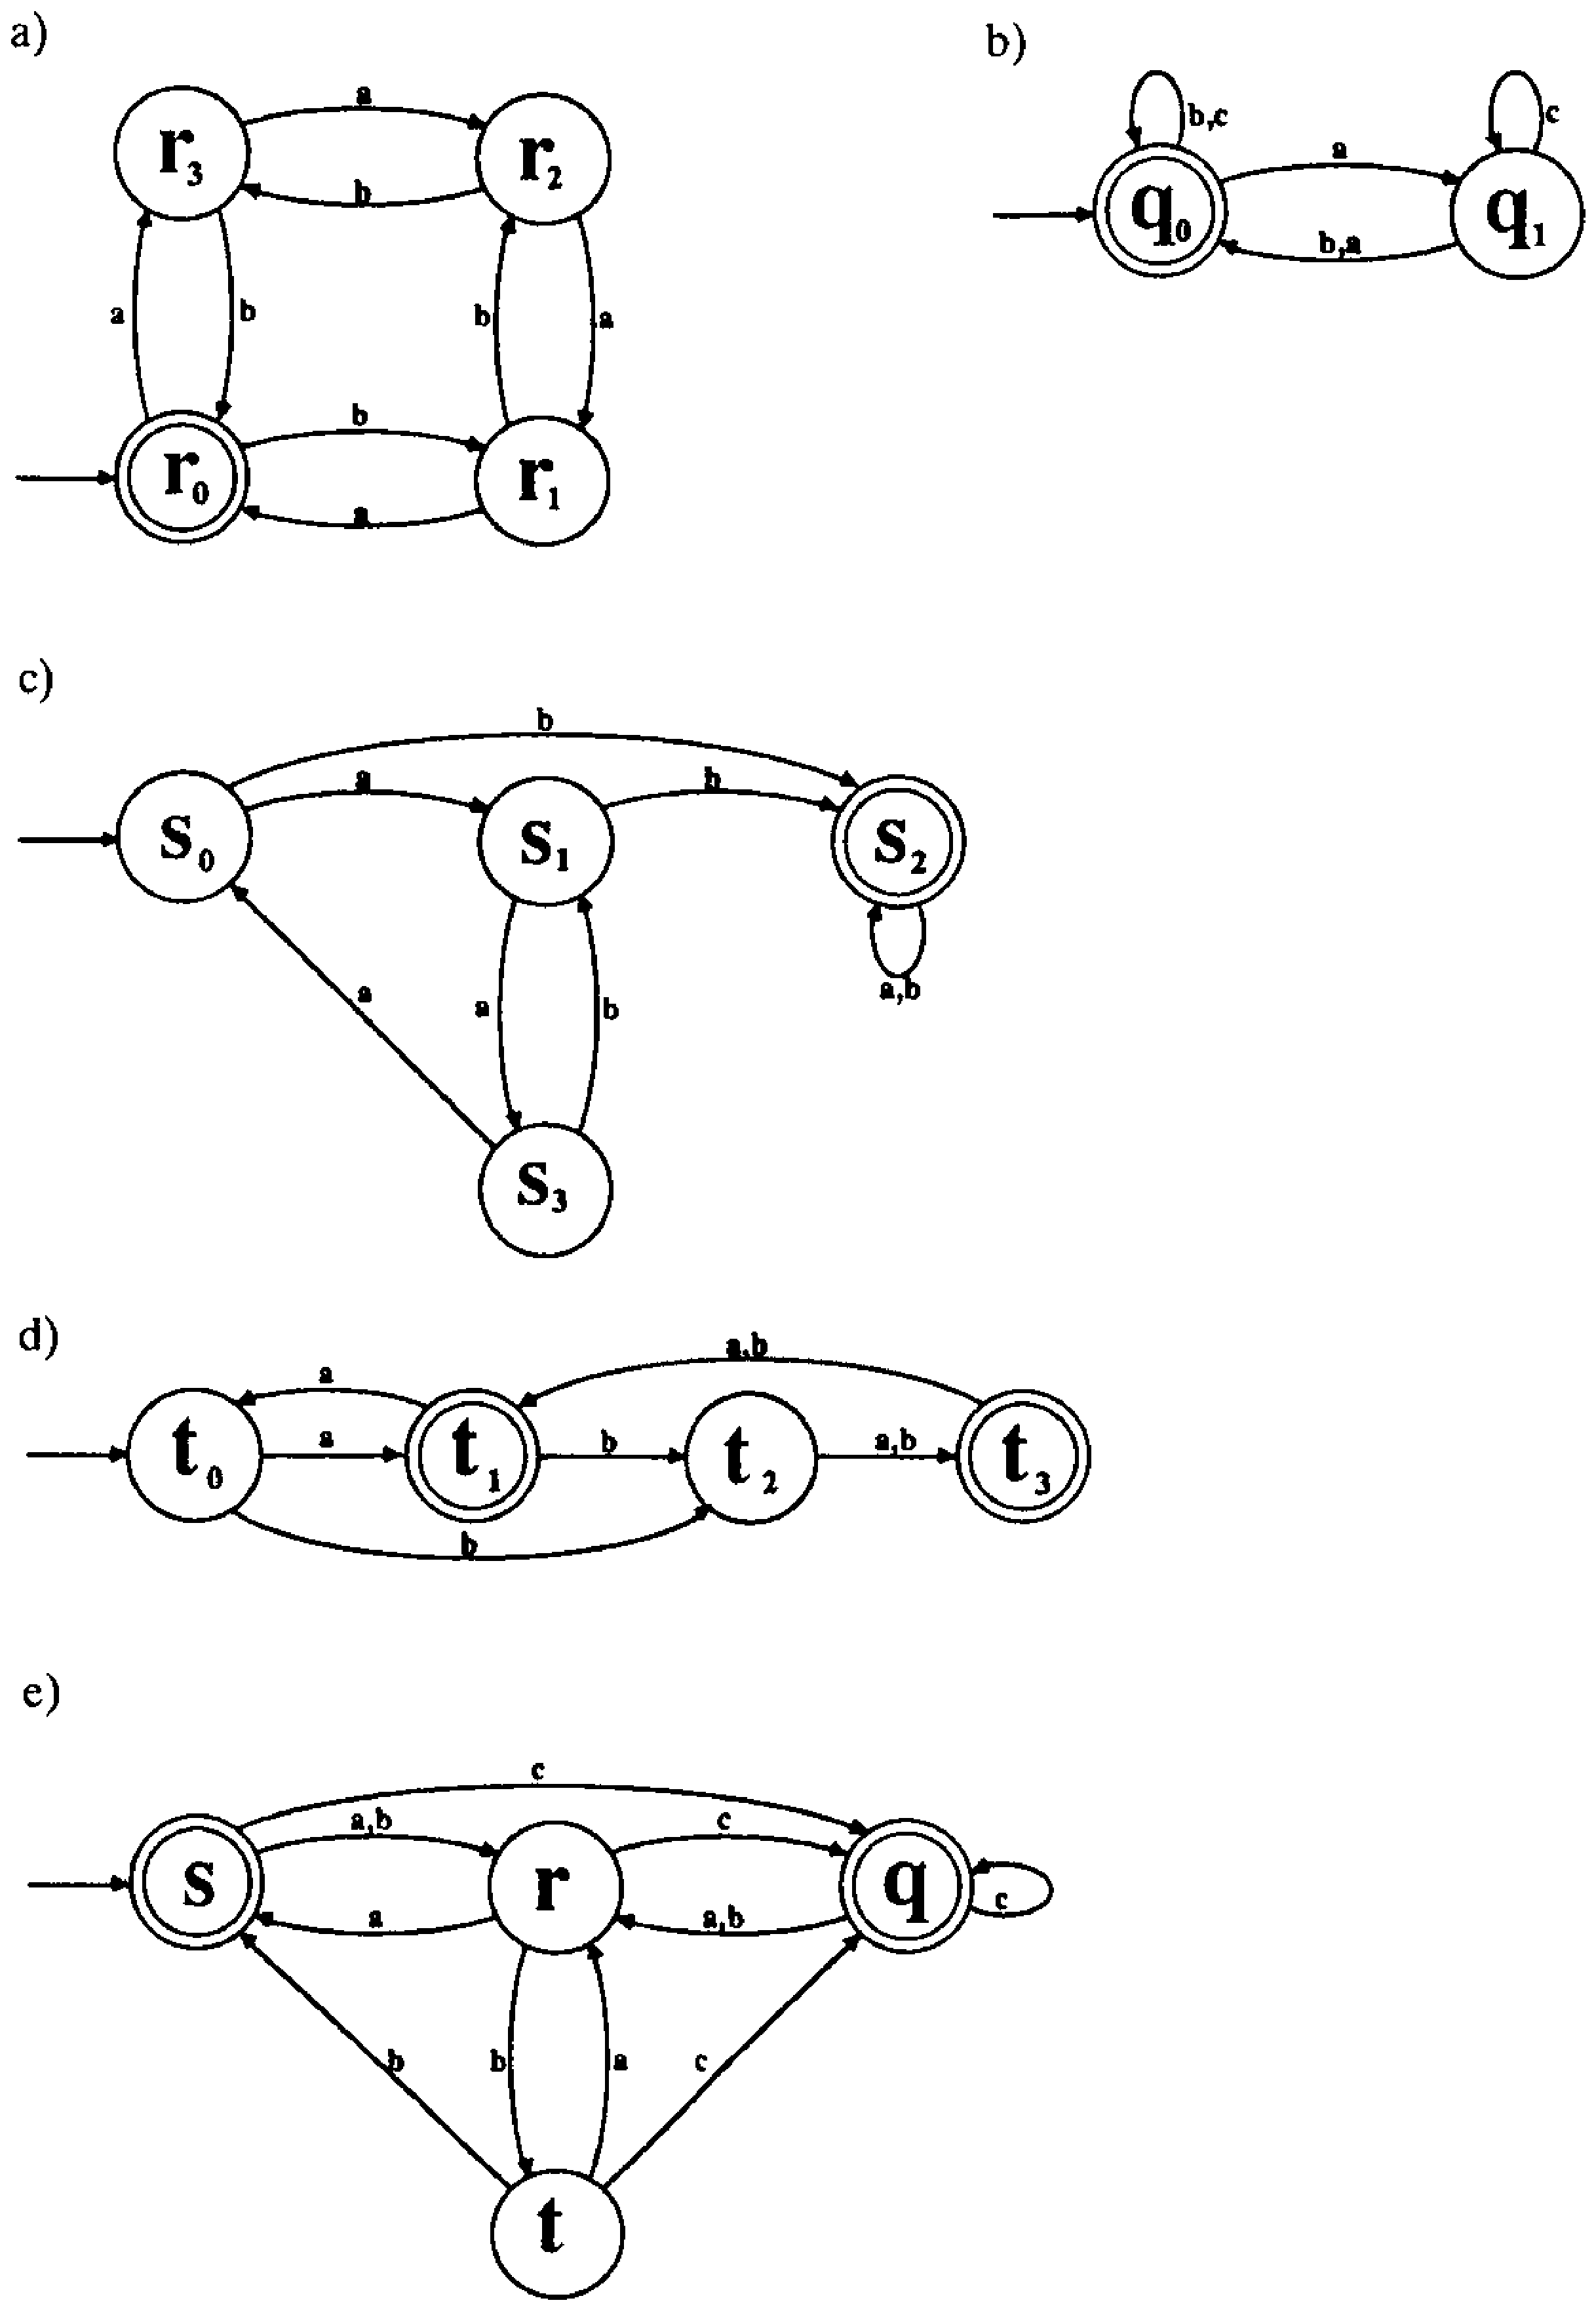
\epsfig{figure=ToFAfigures/fig8-4.eps,width=5.2in}}
\caption{Automata for Exercise 8.31}\label{fig-8.4}
\end{figure}

% Figure 8.5
\begin{figure}
\centerline{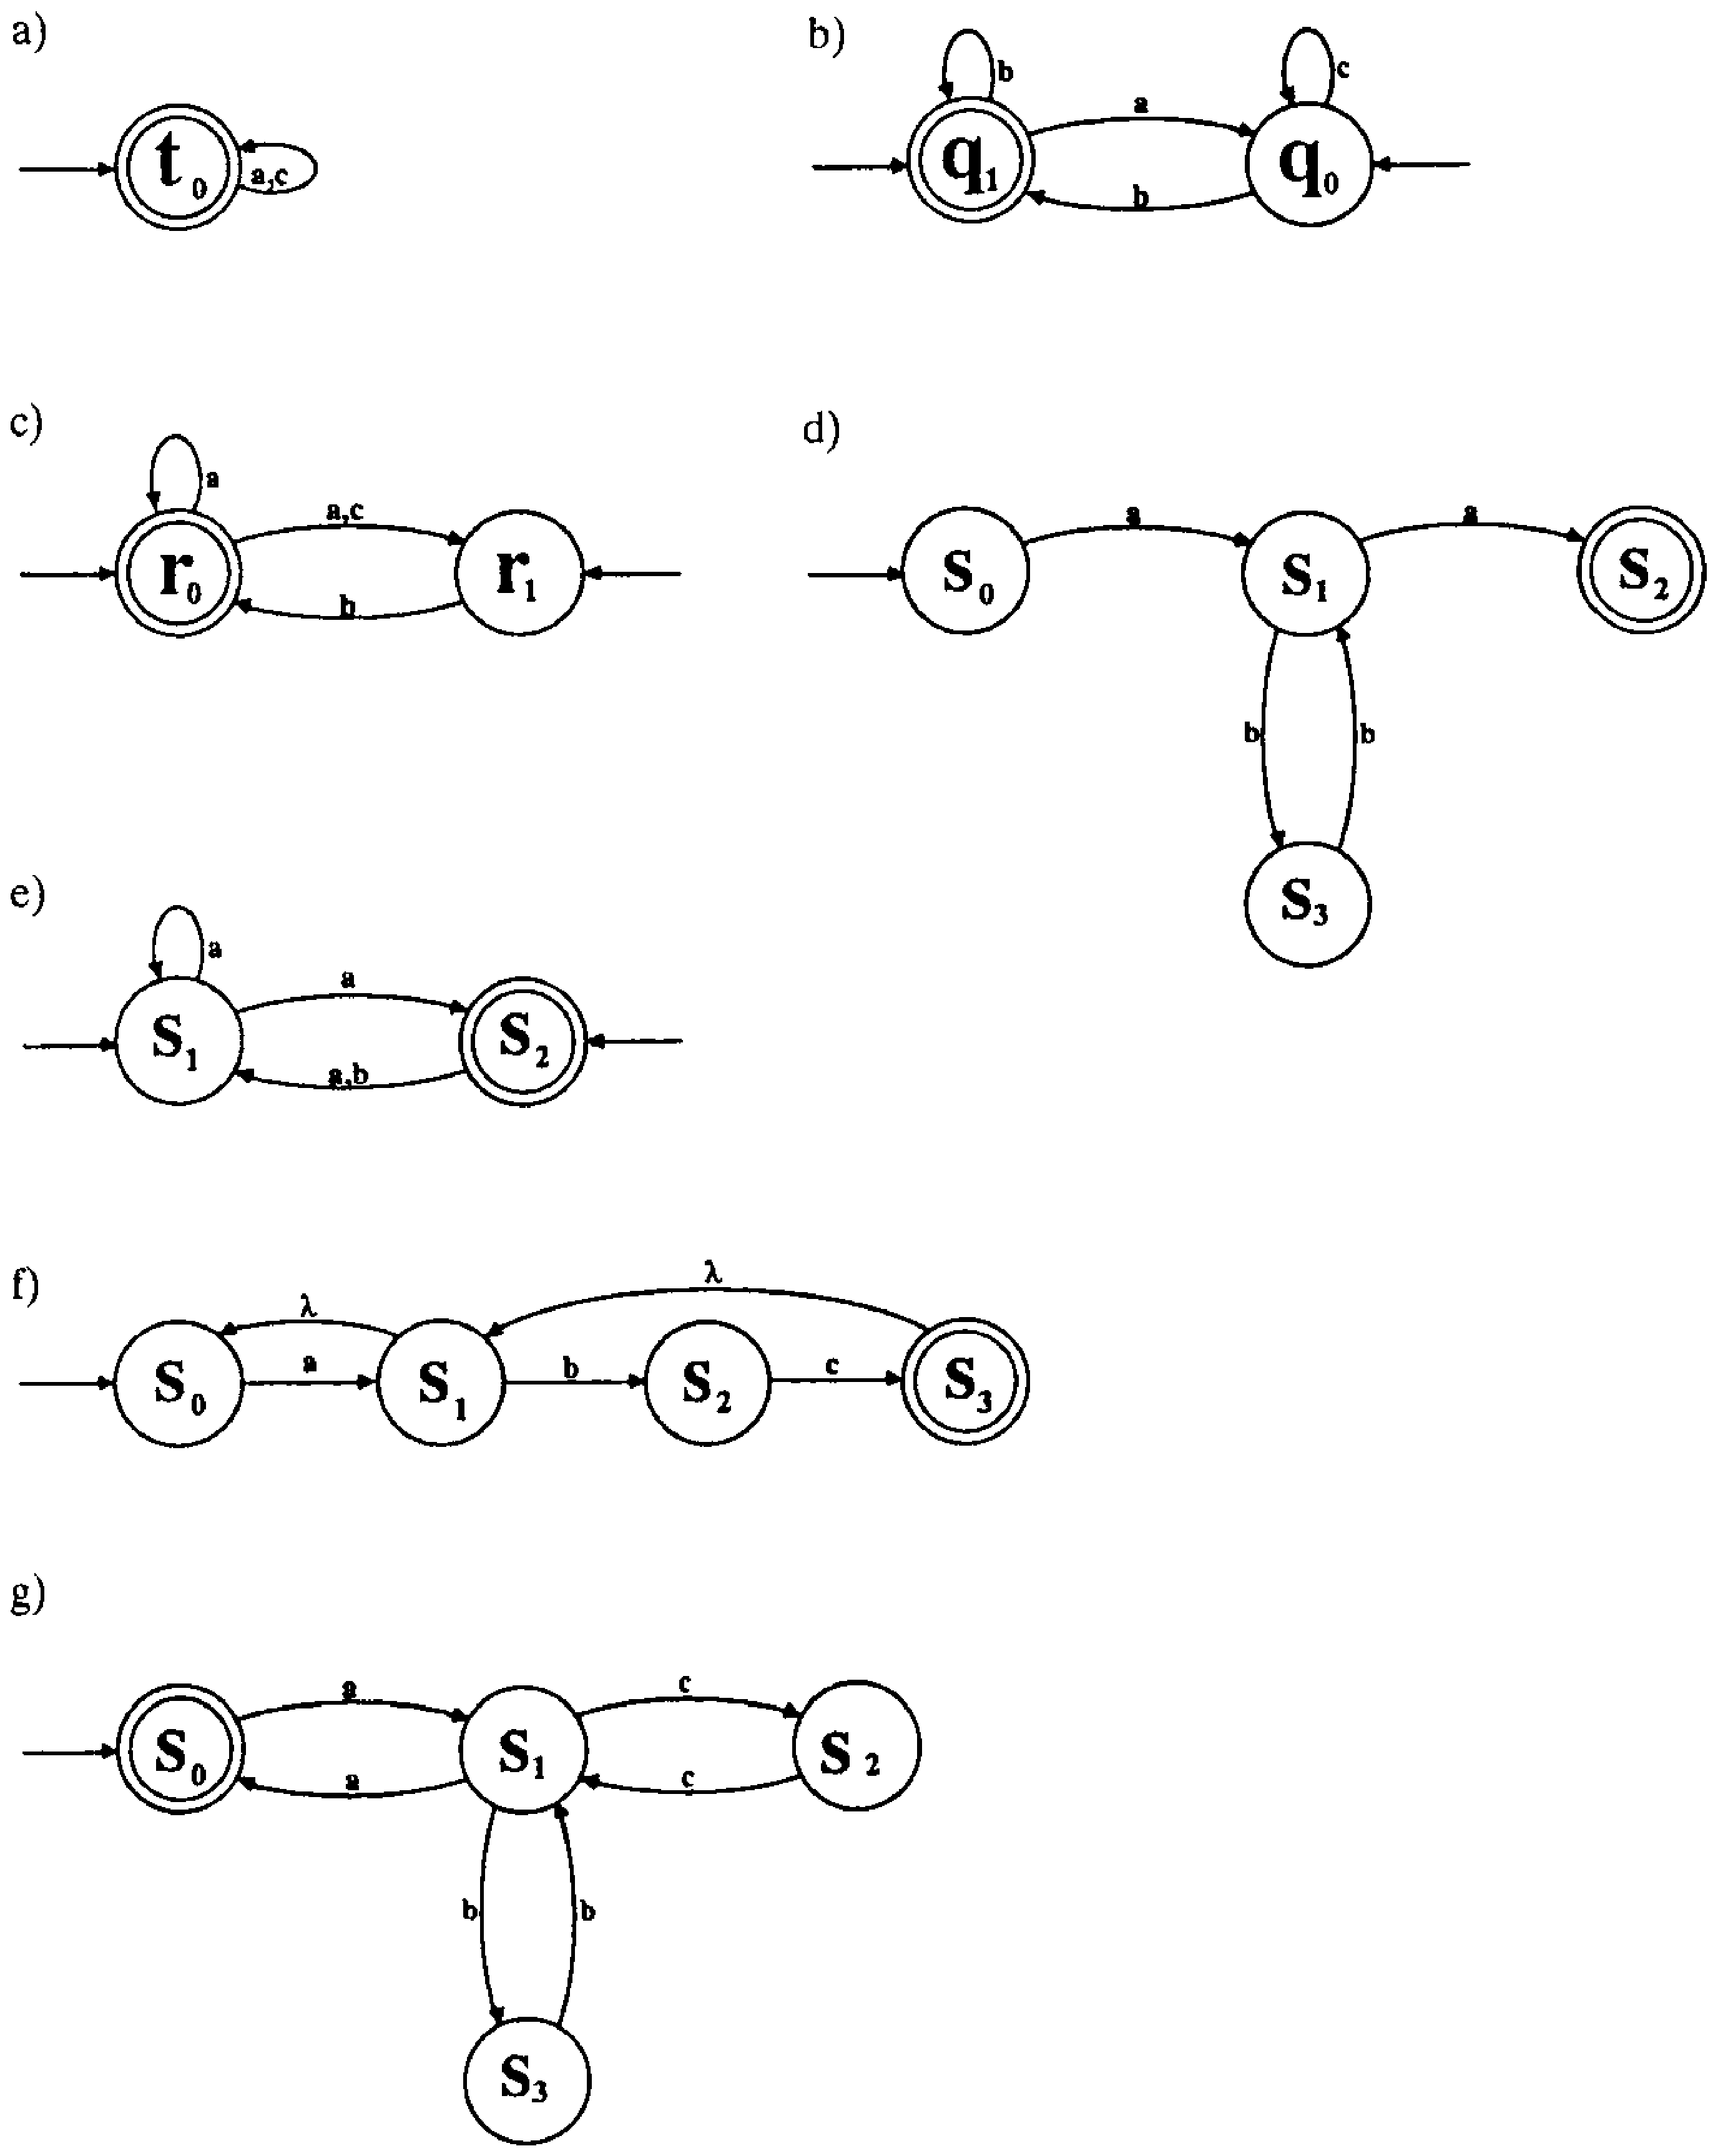
\epsfig{figure=ToFAfigures/fig8-5.eps,width=5.2in}}
\caption{Automata for Exercise 8.32}\label{fig-8.5}
\end{figure}

\item Let $\Sigma=\{\pmb{a},\pmb{b}\}$.  Define context-free grammars for the following languages:
\begin{enumerate}
\item $L_1 =$ all words over $\Sigma^*$ for which the last letter matches the
first letter.
\item $L_2 =$ all odd-length words over $\Sigma^*$ for which the first letter
matches the center letter.
\item $L_3 =$ all words over $\Sigma^*$ for which the last letter matches none
of the other letters.
\item $L_4 =$ all even-length words over $\Sigma^*$ for which the two center
letters match.
\item $L_5 =$ all odd-length words over $\Sigma^*$ for which the center letter
matches none of the other letters.
\item Which of the above languages are regular?
\end{enumerate}

\item Define context-free grammars for the following languages:
\begin{enumerate}
\item $L=\{x\in\{\pmb{a},\pmb{b}\}^*\ |\ \ |x|_a < |x|_b\}$
\item $G=\{x\in\{\pmb{a},\pmb{b}\}^*\ |\ \ |x|_a \geq |x|_b\}$
\item $K=\{w\in\{\pmb{0},\pmb{1}\}^*\ |\ w=w^r\}$
\item $\Phi=\{x\in\{\pmb{a},\pmb{b},\pmb{c}\}^*\ |\ \exists i,j,k\in\NN\ni x =
\pmb{a}^j\pmb{b}^k\pmb{c}^m$, where $j \geq 3$ and $k = m\}$
\end{enumerate}

\item Define context-free grammars for the following languages:
\begin{enumerate}
\item $L_1=\{x\in\{\pmb{a},\pmb{b}\}^*\ |\ \ |x|_a = 2|x|_b\}$
\item $L_2=\{x\in\{\pmb{a},\pmb{b}\}^*\ |\ \ |x|_a \not= |x|_b\}$
\item The set of all postfix expressions over the alphabet $\{\pmb{A},\pmb{B},
\pmb{+},\pmb{-}\}$
\item The set of all parenthesized infix expressions over the alphabet $\{\pmb{A},
\pmb{B},\pmb{+},\pmb{-},\pmb{(},\pmb{)}\}$
\end{enumerate}

\item Define context-sensitive grammars for the following languages:
\begin{enumerate}
\item $\Gamma = \{x\in\{\pmb{0},\pmb{1},\pmb{2}\}^*\ |\ \exists w\in\{\pmb{0},
\pmb{1}\}^*\ni x=w\cdot 2\cdot w\}=\{\pmb{2},\pmb{121},\pmb{020},\pmb{11211},
\pmb{10210},\ldots\}$
\item $\Phi = \{x\in\{\pmb{b}\}^*\ |\ \exists j\in\NN\ni |x|=2^j\}=\{\pmb{b},
\pmb{bb},\pmb{bbbb},\pmb{b}^8,\pmb{b}^{16},\pmb{b}^{32},\ldots\}$
\end{enumerate}

\item Consider the grammar
\[ G=\langle\{A,B,S\},\{\pmb{a},\pmb{b},\pmb{c}\},S,\{S\rightarrow\pmb{a}SB
	\pmb{c},S\rightarrow\lambda,SB\rightarrow\pmb{b}S,\pmb{c}B\rightarrow B
	\pmb{c}\}\rangle \]
Show that this context-sensitive grammar is \emph{not} equivalent to $G''$ given in
Example 8.3, where
\[ G'' = \langle\{A,B,S,T\},\{\pmb{a},\pmb{b},\pmb{c}\},S,\{S\rightarrow\pmb{a}SB
	\pmb{c},S\rightarrow T,T\rightarrow\lambda,TB\rightarrow\pmb{b}T,\pmb{c}
	B\rightarrow B\pmb{c}\}\rangle \]

\item Design context-free grammars that accept:
\begin{enumerate}
\item $L_1=\pmb{a}^*(\pmb{b}\cup\pmb{c})^*\cap\{x\in\{\pmb{a},\pmb{b},\pmb{c}\}^*
\ |\ \ |x|_a = |x|_b + |x|_c\}$
\item $L_2 = \{x\in\{\pmb{a},\pmb{b},\pmb{c}\}^*\ |\ \exists i,j,k\in\NN \ni x =
\pmb{a}^i\pmb{b}^j\pmb{c}^k$, where $i + j = k\}$
\item $L_3 = \{x\in\{\pmb{a},\pmb{b},\pmb{c}\}^*\ |\ \ |x|_a + |x|_b = |x|_c\}$
\end{enumerate}

\item Refer to Definition \ref{dfn-8.4} and prove that $L(G') = L(G) \cup \{\lambda\}$.

\item Refer to Definition \ref{dfn-8.6} and prove that $L(G') = L(G) \cup \{\lambda\}$.

\item \begin{enumerate}
\item Show that if $G$ is in the form specified in Theorem \ref{thm-8.8}, so is the $G_*$ described in
Theorem \ref{thm-8.5}.
\item Give an example that shows that, even if $G_1$ and $G_2$ are in the form
specified in Theorem \ref{thm-8.8}, the grammar $G^{\cup}$ described in Theorem \ref{thm-8.4} may
not be.
\item Is your construction for $G^\bullet$ in Example 8.18 normal form preserving?
\end{enumerate}

\item Given two left-linear grammars $G_1$ and $G_2$, give a set of rules to
find a new left-linear grammar that will generate:
\begin{enumerate}
\item $L(G_1) \cup L(G_2)$
\item $L(G_1)\cdot L(G_2)$
\item $L(G_1)^*$
\end{enumerate}
\end{enumerate}
